\documentclass[notitlepage]{article}
\usepackage{amsmath}
\usepackage{mathtools}
\usepackage{amsthm}
\usepackage{amssymb}
\usepackage{graphicx}
\usepackage{array}
\usepackage{wrapfig}
\usepackage{algorithm}% http://ctan.org/pkg/algorithm
% \usepackage{algorithmic}
\usepackage{algpseudocode}% http://ctan.org/pkg/algorithmicx
\usepackage[utf8]{inputenc}
\usepackage[a4paper, margin=2.5cm, left=3.5cm, right=3.5cm]{geometry}
\usepackage{accents}
\usepackage{float}
\usepackage{hyperref}
\usepackage{bookmark}
\usepackage{multirow}
\usepackage{pdfpages}
\usepackage{subcaption}
\usepackage{sectsty}
\usepackage{ragged2e}
\usepackage{titlesec}
\usepackage{listings}
\usepackage{etoolbox}
\usepackage[outline]{contour}
\usepackage[font=small,skip=1pt]{caption}
\usepackage{enumitem}
\usepackage{tikz}
\usetikzlibrary{arrows}
%Includes "References" in the table of contents
\usepackage[nottoc]{tocbibind}
\usepackage{appendix}
\usepackage{xcolor,colortbl}


\newcommand{\highlight}[1]{{\cellcolor{yellow!30} #1}}

\setlength\parindent{0pt}

\setlength{\tabcolsep}{20pt}
\renewcommand{\arraystretch}{1.5}

\newcolumntype{P}[1]{>{\centering\arraybackslash}p{#1}}
\newcolumntype{M}[1]{>{\centering\arraybackslash}m{#1}}

\algnewcommand\algorithmicforeach{\textbf{for each}}
\algdef{S}[FOR]{ForEach}[1]{\algorithmicforeach\ #1\ \algorithmicdo}

\titleformat{\chapter}[block]
  {\normalfont\huge\bfseries}{\thechapter.}{10pt}{\huge}
\titlespacing*{\chapter}{0pt}{0pt}{10pt}

\makeatletter
\patchcmd{\chapter}{\if@openright\cleardoublepage\else\clearpage\fi}{}{}{}
\makeatother

\newcommand*\circled[1]{\tikz[baseline=(char.base)]{\node[shape=circle,draw,inner sep=2pt] (char) {#1};}}
\newcommand{\ubar}[1]{\underaccent{\bar}{#1}}
\newcommand{\e}[1]{\cdot10^{#1}}
\newtheorem{theorem}{Theorem}[section]
\newtheorem{definition}{Definition}[section]
\newtheorem{lemma}{Lemma}[section]
\newtheorem{corollary}{Corollary}[section]
\newtheorem{proposition}{Proposition}[section]

\DeclareMathOperator*{\argmax}{arg\,max}
\DeclareMathOperator*{\argmin}{arg\,min}

\def\changemargin#1#2{\list{}{\rightmargin#2\leftmargin#1}\item[]}
\let\endchangemargin=\endlist 




\title{Project Non-ML 5\\Final Project for the CM course 2020/21}
\author{Matteo De Francesco}
\date{}
\begin{document}

\maketitle

\thispagestyle{empty}

\tableofcontents

\newpage

\pagenumbering{arabic}

\section{Introduction}
In this report we will analize the convex quadratic problem
\begin{equation}
    \min \left\lbrace x^T Q x + q x : \sum_{i \in I^k} x_i = 1, k\in K, x \ge 0 \right\rbrace
    \label{eqn:problem} \tag{$P$}
\end{equation}
with the following constraints: $x \in \mathbb{R}^n$, the index sets $I^k$ form a partition of the set $\{1,\ldots,n\}$ (i.e.$ \cup_{k\in K} I^k = \{ 1,\ldots,n \}$, and $I^h \cap I^k = \emptyset $ for all
$h$ and $k$), and $Q$ is positive semidefinite.\\
% This is a quadratic problem with a simplicial complex constraint, so the objective, in terms of the primal problem, is finding the x (the simplicial complex) which lies in the minimum of our quadratic function.\\
The aim of this project is to exploit the Lagrangian dual problem and solve it via one of the \textit{deflected subgradient} methods.\\
We can identify the inequality and equality constraints and rewrite them in the typical form
\begin{gather*}
  G(x) \rightarrow g_i(x) \le 0 \implies -x_i \le 0 \ \forall i \in \{1,\ldots,n\} \\
  H(x) \rightarrow h_j(x) = 0 \implies \sum_{i \in I^k} x_i - 1 = 0 \ \forall k \in K
\end{gather*}    
Hence we can rewrite the problem in the following form:
\begin{align*}
  \begin{cases}
    \min\  x^T Q x + q x \\
    -x_i \le 0 \ \forall\, i \in \{1,\ldots,n\} \\
    \sum_{i \in I^k} x_i - 1 = 0 \ \forall\, k \in K
  \end{cases}    
\end{align*}
In order to have less dual variables, we can rewrite the above problem as a lagrangian function of only the inequality constraints:
\begin{align*}
  \mathcal{L}(x;\lambda) = x^T Q x + q^T x + \left\langle \lambda,x \right\rangle 
\end{align*}
% {\large Make the dual function depending only on $\lambda$ and "ignore" the equality constraints $\mu$. In this way the relaxed problem is much more easier since we have only to optimize dual variables $\mu$}.\\
% and then applying the Lagrangian duality we can write the function
% \begin{equation}
%   L(x;\lambda,\mu) = x^T Q x + q x - \sum_{j=1}^n \lambda_j x_j + \sum_{k=1}^{|K|} \left( \mu_k \sum_{i \in I^k} x_i - 1 \right) = x^T Q x + q x - \left\langle \lambda,x \right\rangle + \left\langle \mu,\sum_{i \in I^k} x_i - 1 \right\rangle
% \end{equation}
% where the vector $\lambda \in \mathbb{R}_+^n$ and $\mu \in \mathbb{R}^{|K|}$.\\
Now, we can easily construct the lagrangian dual function considering the equality constraints
\[
  \psi(\lambda) = \min_{x \in \mathcal{Y}} \left\lbrace \mathcal{L}(x;\lambda) ,\ \lambda \ge 0 \right\rbrace
\]
where $\mathcal{Y} = \{\sum_{i \in I^k} x_i = 1 \ \forall\, k \in K\}$. Hence the following optimization problem
\begin{equation}
  \begin{cases}
    \max_{\lambda}\  \psi(\lambda)  \\
    \text{subject to } \lambda \ge 0 
  \end{cases}
  \label{eqn:dual_problem}  
  \tag{$D$}
\end{equation}
We are assuming that optimizing over the set $\mathcal{Y}$ can be done very easily.\\ 
In the next section, we will briefly recall the properties of the \texttt{ADAGRAD} family of algorithms\cite{JMLR:v12:duchi11a}.% and analyze it in our problem setting.

\section{Deflected subgradient Analysis}
% ADAGRAD ANALYSIS
\subsection{\texttt{ADAGRAD} introduction}
The projection rule of a point $y$ onto the constraint set $\mathcal{X}$ according to a positive semidefinite matrix $A$ amounts to:
\[ \prod_\mathbb{X}^A (y) = \argmin_{\lambda \in X} \| \lambda-y \|_A = \argmin_{\lambda \in X} \left\langle \lambda-y,A(\lambda-y) \right\rangle \]
and it's aimed to minimize the Mahalanobis norm.\\
\texttt{ADAGRAD} applies the following projection rule:
\begin{equation}
  \lambda_{t+1} = \prod_\mathcal{X}^{diag(G_t)^{1/2}} (\lambda_t - \eta \, diag(G_t)^{-1/2} g_t) 
  \label{eqn:projection}
\end{equation}
where the matrix $A$ coincides with the diagonal square root of the full outer product of the subgradients $G_t = \sum_{\tau=1}^t g_\tau g_\tau^T$.
% The constraint set $\mathcal{X}$ coincide with the constraints of disjoint simplices, thus resulting 
% in a constraint set coincident with a simplicial complex. So we have to project points of our original quadratic problem onto a simplicial complex .\\
As we stated in the introduction, we should exploit \texttt{ADAGRAD} on the dual problem, whose constraint set consists in the simple inequality constraint $\lambda \ge 0$, which is addressable by \texttt{ADAGRAD},
given the fact that the algorithm can be applied to any convex set $\mathcal{X} \subseteq \mathbb{R}^n$, respected by our problem (we are in $\mathbb{R}_+^n$).\\
In addition, as the general projection rule tell us, the new update $\lambda_{t+1}$ is projected over the constraint set $\mathcal{X}$ according to the matrix of the gradients.\\
% Not only, since we are using the PDSM (primal-dual subgradient methods) update rule inside the \texttt{ADAGRAD} framework, \texttt{LEMMA} 2 of \cite{Frangioni2017} in Appendix A give us a proof of the convergence of the method over the space $\mathbb{R}_+^n$, 
% which coincide exactly with our setting.\\
We will recall in the next section some algorithmic properties of the algorithm convergence for diagonal matrices, and we will derive the update rule followed by the projection over the constraint set $\mathcal{X} = \{\lambda \ge 0\}$.

\subsection{Algorithm characteristics}
First of all, we reiterate that \texttt{ADAGRAD} is suitable for the dual problem, given its application in a convex setting. The goal is to attain a small regret bound:
\begin{equation}
  R_\phi (T) \triangleq \sum_{t=1}^T \psi(\lambda_t) - \psi(\lambda^*)
\end{equation}
between the actual value of the dual function $\psi$ with the corresponding iterate $\lambda$ at step $t$ and the value of $\psi$ with the optimal solution $\lambda^*$.\\
The point of \texttt{ADAGRAD} is that not all features are equal, hence they must be treated differently. That's the purpose of using an adaption to the geometry of space, so do not use anymore a standard gradient descent but conditioning 
the different values based on a positive semidefinite matrix $A$ (the $G_t$ in this case).\\
Two algorithm versions are analyzed in \cite{JMLR:v12:duchi11a}, where we omitted the regularization term due to our problem setting. The first update, referred to as \textit{primal-dual subgradient method}, is 
\begin{equation}
  \lambda_{t+1} = \argmin_{\lambda \in \mathcal{X}} \{ \eta \left\langle \overline{g}_t,\lambda \right\rangle + \frac{1}{t} \Psi_t(\lambda) \}
  \label{eqn:primal-dual-update}
\end{equation}
coming from \cite{NIPS2009_7cce53cf}, where $\overline{g}_t = \frac{1}{t} \sum_{\tau=1}^t g_\tau$ is the average gradient, $\eta$ is a fixed stepsize and $\Psi_t$ is the \textit{proximal term}.\\
The second update instead
\begin{equation}
  \lambda_{t+1} = \argmin_{\lambda \in \mathcal{X}} \{ \eta \left\langle g_t,\lambda \right\rangle + B_{\Psi_t} (\lambda,\lambda_t) \}
  \label{eqn:composite-mirror-update}
\end{equation}
where $B$ refers to the Bregman divergence. This second update comes from \cite{inproceedings}.\\
Finally, also the previous mentioned projection rule can be used as an update:
\begin{equation}
  \lambda_{t+1} = P_{\mathcal{X}} \{ \lambda_t + \eta\, diag(G_t)^{-1/2} g_t \}
  \label{eqn:standard-rule}
\end{equation}
where $P$ denotes the projection operation. The proximal term $\Psi_t$ is the key point of the algorithm. Instead of using a fixed proximal functions, both the updates use squared Mahalanobis norms as their proximal functions, setting then $\Psi_t(\lambda) = \left\langle \lambda,H_t \lambda \right\rangle$ 
for a symmetric matrix $H_t \succeq 0$. In particular, the diagonal case which we will recall here make use of:
\[ H_t = \delta I + diag(G_t)^{1/2} \]
for some smalled fixed $\delta \ge 0$.\\
The usage of a strongly convex proximal function is also remarked in \cite{Frangioni2017} in appendix A.

\subsection{Proximal term discussion}
In order to attain a lower regret bound and to adapt to the geometry of the space, the objective of the authors is to not use anymore a standard proximal functions but a modified version of it.\\
The proximal function act as a regularization term, typically the Euclidian projection over a convex set. Given the indicator function of a convex set $C$:
\begin{align*}
  I_C(\lambda) = \begin{cases}
    0 \quad \lambda \in C \\
    +\infty \quad \text{otherwise}
  \end{cases}
\end{align*}
the standard proximal mapping of $I_C$ is the Euclidean projection on $C$:
\begin{align*}
  prox_{I_C}(\lambda) = \argmin_{u \in C} \| u - \lambda \|_2^2 = P_C(\lambda)
\end{align*}
Instead in this case the authors noticed that some local region of the function to be optimized need more "attention than others". What they come up with then is the modification (also remarked in the \texttt{ADAGRAD} introduction) using a different proximal function where  
\begin{align*}
  prox_{I_C}(\lambda) = \argmin_{u \in C} \| u - \lambda \|_A^2 = P_C(\lambda)
\end{align*}
the Euclidean projection is not computed anymore according to a 2-norm, but according to a matrix $A$ which in the case of \texttt{ADAGRAD} coincide with the matrix of the subgradients. A summary of the properties and aspects of some proximal functions 
can be found in \cite{OPT-003}. Below is reported the analysis of the proximal function regarding \cite{JMLR:v12:duchi11a}.\\
Examining the regret bounds for the updates in \cite{Nesterov2009} and \cite{NIPS2009_7cce53cf}, it is quite obvious that they depends on dual norms of the derivative of the function to be optimized, and in turn this last depend on the choice of $\Psi$. The objective of \cite{JMLR:v12:duchi11a} 
is to properly modify the value of $\Psi$ during the run of the algorithm in order to lower the contribution of the norms, and so lower the regret bound. This is achieved by keeping second order information about the sequence of iterates $\lambda_t$ and allow $\Psi$ 
to vary on each round of the algorithm. To achieve this, we must assume that $\Psi_t$ is monotically non-decreasing, 1-strongly convex with respect to a time-dependent semi-norm $\|\cdot\|_{\Psi_t}$. Formally, given two generic points $x$ and $y$, $\Psi$ is 1-strongly convex with respect 
to $\|\cdot\|_\Psi$ if
\[ \Psi(y) \ge \Psi(x) + \left\langle \nabla \Psi(x),y-x \right\rangle + \frac{1}{2} \|x-y\|_\Psi^2 \]
As a consequence, strong convexity is guaranteed if and only of $B_{\Psi_t}(x,y) \ge \frac{1}{2} \|x-y\|_{\Psi_t}^2$. The following bound holds then on proximal term, respectively for \eqref{eqn:primal-dual-update} and \eqref{eqn:composite-mirror-update}. 
Proofs can be found in Appendix F of \cite{JMLR:v12:duchi11a}.
\begin{proposition}
  Let the sequence $\{\lambda_t\}$ be defined by the update \eqref{eqn:primal-dual-update}. For any $\lambda^* \in \mathcal{X}$
  \begin{equation}
    \sum_{t=1}^T \psi(\lambda_t) - \psi(\lambda^*) \le \frac{1}{\eta} \Psi_T(\lambda^*) + \frac{\eta}{2} \sum_{t=1}^T \| \psi'(\lambda_t) \|_{\Psi_{t-1}^*}^2
  \end{equation}
\end{proposition}
\begin{proposition}
  Let the sequence $\{\lambda_t\}$ be defined by the update \eqref{eqn:composite-mirror-update}. For any $\lambda^* \in \mathcal{X}$
  \begin{align*}
    \sum_{t=1}^T \psi(\lambda_t) - \psi(\lambda^*) \le \frac{1}{\eta} B_{\Psi_1} (\lambda^*,\lambda_1) + \frac{1}{\eta} \sum_{t=1}^{T-1} \left[ B_{\Psi_{t+1}}(\lambda^*,\lambda_{t+1}) - B_{\Psi_t}(\lambda^*,\lambda_{t+1}) \right] \\ + \frac{\eta}{2} \sum_{t=1}^T \| \psi'(\lambda_t) \|_{\Psi_t^*}^2
  \end{align*}
\end{proposition}
The proximal term and the bregman divergence present in \eqref{eqn:primal-dual-update} and \eqref{eqn:composite-mirror-update} will be computed according to the subgradient matrix, in order to iteratively modify the update and thus adapting to the 
geometry of the space.
% \\[1em]
% Proximal term allows us to build upon the surface of our function, starting from the first order derivative according to Taylor's rule, we build a "parabola" (a strongly convex function in general) using the euclidean norm according to the matrix. In this way, we 
% explore the different "parabolas" over the derivative and according to this we choose the minimum $x$ which give us the $\arg\min$. (?)

\subsection{Convergence Analysis}
\label{sec:convergence}
First of all, let us state that the convergence rate of \texttt{ADAGRAD} is the same of the Stochastic Gradient Descent (\texttt{SGD}), hence $O(1/\sqrt{T})$ but with a lower constant due to the use of $G$ matrix.\\
The algorithm 1 reported in \cite{JMLR:v12:duchi11a} will be applied to our problem and is reported here:
\begin{algorithm}[H]
  \caption{\texttt{ADAGRAD} for diagonal matrices}
  \label{alg:adagrad}
  \begin{algorithmic}
    \Function{\texttt{ADAGRAD}}{$\eta$,$\delta$}
      \State $x_1 \gets 0$
      \State $\lambda_1 \gets 0$
      \State $g_{1:0} \gets \left[\,\right]$
      \For{$t \gets 1$ to $T$}
        \State $Loss = f_t(x_t)$
        \State $g_t \gets \partial \psi(\lambda_{t-1})$ of $\psi$ at $\lambda_{t-1}$\Comment{Compute subgradient at $\lambda_{t-1}$}
        \State $g_{1:t} \gets \left[ g_{1:t-1}\ g_t \right]$\Comment{Store subgradient}
        \State $s_{t,i} \gets \| g_{1:t,i} \|_2$\Comment{Compute the optimal $s_{t,i}$}
        \State $H_t \gets \delta \mathit{I} + diag(s_t)$
        \State $\Psi_t(\lambda) \gets \frac{1}{2} \left\langle \lambda,H_t \lambda \right\rangle$
        \State Either compute \eqref{eqn:primal-dual-update} or \eqref{eqn:composite-mirror-update} 
      \EndFor
    \EndFunction
  \end{algorithmic}  
\end{algorithm}
The general convergence result of this algorithm for both the updates is reported in theorem 5 of the original paper. We will now report the theoretical analysis behind procedure \ref{alg:adagrad} and lastly modify the algorithm in order to match our problem settings.
\begin{theorem}
  Let the sequence $\{\lambda_t\}$ be defined by algorithm \ref{alg:adagrad}. For $\lambda_t$ generated using the update \eqref{eqn:primal-dual-update} with $\delta \ge \max_t \|g_t\|_\infty$, for any $\lambda^* \in \mathcal{X}$
  \begin{equation} 
    R_\phi(T) \le \underbrace{\frac{\delta}{\eta} \|\lambda^*\|_2^2 + \frac{1}{\eta} \|\lambda^*\|_\infty^2 \sum_{i=1}^d \|g_{1:T,i}\|_2}_{\text{\circled{1}}} + \underbrace{\eta \sum_{i=1}^d \|g_{1:T,i}\|_2}_{\text{\circled{2}}} 
    \label{eqn:pd-regret}
  \end{equation}
  For $\lambda_t$ generated using the update \eqref{eqn:composite-mirror-update}, for any $\lambda^* \in \mathcal{X}$
  \begin{equation}
    R_\phi(T) \le \underbrace{\frac{1}{2\eta} \max_{t \le T} \|\lambda^* - \lambda_t\|_\infty^2 \sum_{i=1}^d \|g_{1:T,i}\|_2}_{\text{\circled{3}}} + \underbrace{\eta \sum_{i=1}^d \|g_{1:T,i}\|_2}_{\text{\circled{2}}} 
    \label{eqn:cm-regret}  
  \end{equation}
  \label{th:regrets}
\end{theorem}
We will now delve into analyzing the different \circled{$\cdot$} parts.\\
First of all, we should recall some intuition in order to understand better the regret bound provided above.\\
Focusin on the algorithm \ref{alg:adagrad}, the chosen value of $s_{t,i}$ explain us why the particular choice of the proximal function $\Psi_t(x) = \frac{1}{2} \left\langle x,H_t x \right\rangle$ is so important. $s_{t,i}$ comes from the solution of the problem
\[ \min_s \sum_{t=1}^T \sum_{i=1}^d \frac{g_{t,i}^2}{s_i} \text{ s.t. } s \succeq 0, \left\langle 1,s \right\rangle \le c \] 
solved by optimizing the Lagrangian
\[ 
  \mathcal{L}(s,\lambda,\theta) = \sum_{i=1}^d \frac{\| g_{1:T,i} \|_2^2}{s_i} - \left\langle \lambda,s \right\rangle + \theta (\left\langle 1,s \right\rangle - c ) 
\]
Taking the partial derivatives to find the infimum of $\mathcal{L}$, and using the complementary slackness condition on $\lambda_i s_i$ imply that $\lambda_i = 0$. As a consequence, we obtain $s_i = c \| g_{1:T,i} \|_2 / \sum_{j=1}^d \| g_{1:T,j} \|_2$.
Plugging this into the previous objective function, we get
\[ \inf_s \left\lbrace \sum_{t=1}^T \sum_{i=1}^d \frac{g_{t,i}^2}{s_i} : s \succeq 0, \left\langle 1,s \right\rangle \le c \right\rbrace = \frac{1}{c} \left(\sum_{i=1}^d \| g_{1:T,i} \|_2 \right)^2  \]
Now it is natural to suspect that for $s$ achieving the infimum in this latter equation, using a proximal function similar to $\Psi(\lambda) = \left\langle \lambda,diag(s) \lambda \right\rangle$ with associated squared dual norm $\|\lambda\|_{\Psi^*}^2 = \left\langle \lambda,diag(s)^{-1}\lambda \right\rangle$ we should 
lower the gradient terms both in \eqref{eqn:pd-regret} and \eqref{eqn:cm-regret}.\\
The upper bound on the gradient term for both the updates is taken from the \texttt{LEMMA 4} of \cite{JMLR:v12:duchi11a}, stating:
% \begin{lemma}
%   Let $g_t = f_t'(x_t)$ and $g_{1:t}$ and $s_t$ be defined as in algorithm \ref{alg:adagrad}. Then 
%   \[ \sum_{t=1}^T \left\langle g_t,diag(s_t)^{-1}g_t \right\rangle \le 2 \sum_{i=1}^d \|g_{1:t,i}\|_2 \]
% \end{lemma}
\begin{lemma}
  Let $g_t = \psi'(\lambda_t)$ and $g_{1:t}$ and $s_t$ be defined as in algorithm \ref{alg:adagrad}. Then 
  \[ \sum_{t=1}^T \left\langle g_t,diag(s_t)^{-1}g_t \right\rangle \le 2 \sum_{i=1}^d \|g_{1:T,i}\|_2 \]
\end{lemma}
To obtain a bound, we need to consider the terms consisting of the dual-norm of the subgradient in the bounds \eqref{eqn:pd-regret} and \eqref{eqn:cm-regret}, which is $\|\psi'(\lambda_t)\|_{\Psi_t^*}^2$. When we choose $\Psi_t(\lambda) = \left\langle \lambda,(\delta I + diag(s_t)) \lambda \right\rangle$, the associated dual norm is
\[ \| g \|_{\Psi_t^*}^2 = \left\langle g,(\delta I + diag(s_t))^{-1} g \right\rangle\]
Following from the definition of $s_t$ in \ref{alg:adagrad}, we have $\|\psi'(\lambda_t)\|_{\Psi_t^*}^2 \le \left\langle g_t, diag(s_t)^{-1} g_t \right\rangle$. Thus we have the following implication
\[ \sum_{t=1}^T \|\psi'(\lambda_t)\|_{\Psi_t^*}^2 \le \sum_{i=1}^d \|g_{1:T,i}\|_2 \]
which prove the regret term \circled{2}.\\
%QUIQUI
Consequently, it remains to prove the bound over the Bregman divergence and the term $\Psi_T(\lambda^*)$ of proposition 2.1 and 2.2. Focusing on the composite mirror descent, we have:
\begin{align*}
  B_{\Psi_{t+1}} (\lambda^*, \lambda_{t+1}) - B_{\Psi_{t}} (\lambda^*, \lambda_{t+1}) = \frac{1}{2} \left\langle \lambda^* - \lambda_{t+1}, diag(s_{t+1} - s_t)(\lambda^* - \lambda_{t+1}) \right\rangle \\
  \le \frac{1}{2} \max_i (\lambda_i^* - \lambda_{t+1,i})^2 \| s_{t+1} - s_t \|_1
\end{align*}
Since $\| s_{t+1} - s_t \|_1 = \left\langle s_{t+1} - s_t, 1 \right\rangle$ and $\left\langle s_T,1 \right\rangle = \sum_{i=1}^d \| g_{1:T,i} \|_2$ we have
\begin{align*}
  \sum_{t=1}^{T-1} B_{\Psi_{t+1}} (\lambda^*, \lambda_{t+1}) - B_{\Psi_{t}} (\lambda^*, \lambda_{t+1}) \le \frac{1}{2} \sum_{t=1}^{T-1} \| \lambda^* - \lambda_{t+1} \|_\infty^2 \left\langle s_{t+1} - s_t, 1 \right\rangle \\
  \le \frac{1}{2} \max_{t \le T} \|\lambda^* - \lambda_t\|_\infty^2 \sum_{i=1}^d \|g_{1:T,i}\|_2 - \frac{1}{2} \|\lambda^* - \lambda_1\|_\infty^2 \left\langle s_1,1 \right\rangle
\end{align*} 
which prove us the term \circled{3}.\\
Finally, we also have that
\[ \Psi_T(\lambda^*) = \delta \|\lambda^*\|_2^2 + \left\langle \lambda^*, diag(s_T) \lambda^* \right\rangle \le \delta \|\lambda^*\|_2^2 + \|\lambda^*\|_\infty^2 \sum_{i=1}^d \|g_{1:T,i}\|_2 \]
which give us the bound \circled{1}.\\
Performing a few algebraic simplification lead us to a corollary which give us a more intuitive form of the regret bound. Assume that $\mathcal{X}$ is a compact set and set $D_\infty = \sup_{\lambda \in \mathcal{X}} \| \lambda - \lambda^* \|_\infty$, and define
\[ \gamma_T \triangleq \sum_{i=1}^d \| g_{1:T,i} \|_2 = \inf_s \left\lbrace \sum_{t=1}^T \left\langle g_t,diag(s)^{-1} g_t \right\rangle : \left\langle 1,s \right\rangle \le \sum_{i=1}^d \| g_{1:T,i} \|_2, s \succeq 0 \right\rbrace \]
\begin{corollary}
  Assume that $D_\infty$ and $\gamma_T$ are defined as above. For $\{ \lambda_t \}$ generated using the \eqref{eqn:primal-dual-update} with $\eta = \|\lambda^*\|_\infty$, for any $\lambda^* \in \mathcal{X}$ we have
  \begin{align*}
    R_\phi(T) \le 2 \|\lambda^*\|_\infty \gamma_T + \delta \frac{\|\lambda^*\|_2^2}{\|\lambda^*\|_\infty} \le 2 \|\lambda^*\|_\infty \gamma_T + \delta \|\lambda^*\|_1
  \end{align*}
  Using update \eqref{eqn:composite-mirror-update} to generate $\{\lambda_t\}$ and setting $\eta = D_\infty / \sqrt{2}$, we have
  \begin{align*}
    R_\phi(T) \le \sqrt{2} D_\infty \sum_{i=1}^d \| g_{1:T,i} \|_2 = \sqrt{2} D_\infty \gamma_T \\[1em]
  \end{align*}
\end{corollary}
% Consequently, also upper bound for the proximal term and the bregman divergence are obtained in chapter 3 of \cite{JMLR:v12:duchi11a}. Putting together the last lemma result and the proximal terms bounds give us the theorem \ref{th:regrets}. Stated in simpler 
% terms, the goal of the authors is to achieve an asymptotically sub-linear regret, hence having $R_\phi(T) = o(T)$.\\[1em]
All these presented results are respected by our problem. Indeed, as we stated before, our original problem is for sure a convex problem (a quadratic function with positive semidefinite $Q$) and also the constraints are convex (a set of disjoint 
unitary simplices) implying strong duality. As we know from theory, the dual problem is for sure convex, even if the original one it's not. What we should argue is the presence of the constraints on the dual variables.\\
Being \texttt{ADAGRAD} applicable to any convex set $\mathcal{X} \subseteq \mathbb{R}^n$, this is suitable for our problem, since $\mathcal{X} = \{\lambda \ge 0\}$. We will use one of the just explained update, (preferably 
the \textit{primal-dual} one, since we have a general proof of convergence over exactly $\mathbb{R}_+^n$, in \texttt{LEMMA 2} of Appendix A of \cite{Frangioni2017}), compute the update and then project it on the $\lambda$'s constraint set.\\
We expect to achieve an asymptotically sub-linear regret, as the authors showed in their work.


\subsection{General application to our case}
In our setting, we aim to solve problem \eqref{eqn:problem} using \eqref{eqn:dual_problem}. We will use $\mathcal{X} = \{ \lambda \ge 0 \}$ as the constraint set of the lagrangian multipliers $\lambda$'s, and $\mathcal{Y} = \{ \sum_{i \in I^k} x_i = 1 \ \forall \, k \in K\}$ 
as the constraint set of the primal variables.\\
To solve the problem \eqref{eqn:primal-dual-update} and \eqref{eqn:composite-mirror-update} in our problem settings, we consider the update of the dual variable $\lambda$. Referring to the problem \eqref{eqn:dual_problem}, we can freely choose  
among three different update rules, in order \eqref{eqn:projection}, \eqref{eqn:primal-dual-update} and \eqref{eqn:composite-mirror-update}:
\begin{equation}
  \begin{gathered}
    \lambda_{t+1} = P_{\mathcal{X}} \{ \lambda_t + \eta\, diag(G_t)^{-1/2} g_t \} \\
    \lambda_{t+1} = \argmax_{\lambda \in \mathcal{X}} \{ \eta \left\langle \overline{g}_t,\lambda \right\rangle + \frac{1}{t} \Psi_t(\lambda) \} \\
    \lambda_{t+1} = \argmax_{\lambda \in \mathcal{X}} \{ \eta \left\langle g_t,\lambda \right\rangle + B_{\Psi_t} (\lambda,\lambda_t) \}
    \label{eqn:updates}  
  \end{gathered}
\end{equation}
We need to find a maximum for the considered update function and then project it onto the constraint set $\mathcal{X}$.\\
About the terms $\Psi$ and $B_\Psi$, these will be replaced, according to what we have said before,respectively by:
\begin{gather*}
  \Psi_t(\lambda) = \frac{1}{2} \left\langle \lambda,H_t \lambda \right\rangle \\
  B_{\Psi_t} (\lambda,\lambda_t) = \Psi_t(\lambda) - \Psi_t(\lambda_t) - \left\langle \nabla \Psi_t(\lambda_t),\lambda-\lambda_t \right\rangle
\end{gather*}
Regarding the maximum, this can be simply solved by differentiating the function with respect to the variable to be maximized, and setting it equal to $0$. The detailed derivation of each update can be found in the appendix \ref{sec:appendix}.
\begin{subequations}
  \label{eqn:minimized}
  \begin{align}
    \hat{\lambda}_{t+1} = \lambda_t + \eta diag(G_t)^{-1/2} g_t 
    \tag{Update \eqref{eqn:standard-rule}} \\
    \hat{\lambda}_{t+1} = -H_t^{-1} t\, \eta\, \overline{g}_t
    \tag{Update \eqref{eqn:primal-dual-update}} \\
    \hat{\lambda}_{t+1} = \lambda_t + \eta\, H_t^{-1}\, g_t 
    \tag{Update \eqref{eqn:composite-mirror-update}}
  \end{align}
\end{subequations}

For the stepsize $\eta$, this can be fixed apriori and we will see being it crucial for the convergence of the algorithm. Different stepsize rules can be employed \cite{stepsizes}

\begin{align*}
  \eta = h && \text{Constant step size rule, with $h > 0$} \\
  \eta = \frac{h}{\| g^t \|} && \text{Constant step length} \\
  \eta = \frac{\alpha}{\beta + t} && \text{Square summable but not summable, with $\alpha > 0$ and $\beta \ge 0$} \\
  \eta = \frac{\alpha}{\sqrt{t}} && \text{Nonsummable diminishing} \\
  \eta = \frac{f(x^*) - \phi(\lambda_t)}{\|g^t\|^2} && \text{Polyak stepsize} 
\end{align*}

For the dual variables, after we obtain $\hat{\lambda}_{t+1}$, we use the projection over the nonnegative orthant to get $\lambda_{t+1}$, formally
\[
  \lambda_{t+1} = P_\mathcal{X}(\hat{\lambda}_{t+1}) = \max{ \{ 0,\hat{\lambda}_{t+1} \} }
\]
which is a trivial problem tackled many times in the literature \cite{nonnegative-orthant}.\\
% Projection over non negative orthant is a trivial problem and is solved by simply maximizing componentwise $\lambda_t$ between $\left[ 0,P_\mathcal{X}(\hat{\lambda}_t) \right]$ (FORSE NON PROPRIO, LA PROIEZIONE NON È EUCLIDEA MA IN BASE ALLA MATRICE $G$).\\
We need also to derive an update for the primal variables, which are needed at each iteration in order to compute the dual function $\psi( \lambda )$ and the subgradient $\nabla_\lambda \psi( \lambda )$. Given the previous multiplier value $\lambda_t$
\[
  x_{t+1} = \argmin_{x \in \mathcal{Y}} \{ x^T Q x + q^T x + \left\langle \lambda_t,x \right\rangle \}
\]
We need to solve the lagrangian relaxation of a convex quadratic problem, depending on equality constraints made up of disjoint simplices. The constraint set $\mathcal{Y}$ can be rewritten in a matrix form $Ax = b$, where the vector $b$ is a $k \times 1$ vector of all ones, and the matrix $A$
can be derived with the following simple algorithm:
\begin{algorithm}[H]
  \caption{Construct matrix $A$}
  \begin{algorithmic}
    \Procedure{Construct\_$A$}{$K,\left[I^k\right]$}
      \State $A \gets \left[\,\right]$\Comment{Initialize $k \times n$ empty matrix}
      \For{$k \gets 1$ to $K$}
        \State $a_k \gets zeros(n,1)$\Comment{$n \times 1$ empty row vector}
        \For{$i \gets 1$ to $n$}
          \If{$i \in I^k$}\Comment{Check if index $i$ is in the set $I^k$}
            \State $a_k[i] \gets 1$
          \EndIf
        \EndFor
        \State $A[k,:] \gets a_k$
      \EndFor
    \EndProcedure
  \end{algorithmic}
\end{algorithm}
Using the {\bf KKT} (Karush-Kuhn Tucker) conditions, we can solve the problem directly through linear algebra by constructing the following linear system:
\begin{gather*}
  \begin{cases}
    Q x + q - \lambda_t + \mu A = 0 \\
    A x - b = 0
  \end{cases}
  \boldsymbol{\implies} 
  \begin{cases}
    Q x + \mu A = \lambda_t - q \\
    A x \quad \quad \:\ \,= b 
  \end{cases}
  \boldsymbol{\implies} \\ 
  \begin{bmatrix}
    Q & A^T \\[1ex]
    A & 0 
  \end{bmatrix}
  \begin{bmatrix}
    x \\[1ex]
    \mu
  \end{bmatrix}
  = 
  \begin{bmatrix}
    \lambda_t - q \\[1ex]
    b
  \end{bmatrix}
\end{gather*}
a linear system that can be solved directly and efficiently by computing the pivoted LU factorization of the matrix and save it for the next iterations. Hence, using the LU factorization:
\begin{gather*}
  \begin{bmatrix}
    Q & A^T \\[1ex]
    A & 0 
  \end{bmatrix} 
  \begin{bmatrix}
    x \\[1ex]
    \mu
  \end{bmatrix}
  = 
  \begin{bmatrix}
    \lambda_t - q \\[1ex]
    b
  \end{bmatrix}
  \boldsymbol{\implies} 
  \begin{bmatrix}
    x \\[1ex]
    \mu
  \end{bmatrix}
  = 
  \begin{bmatrix}
    Q & A^T \\[1ex]
    A & 0 
  \end{bmatrix}^{-1}
  \begin{bmatrix}
    \lambda_t - q \\[1ex]
    b
  \end{bmatrix}
  \boldsymbol{\implies} \\
  \begin{bmatrix}
    x \\[1ex]
    \mu
  \end{bmatrix}
  = 
  U^{-1} * \left(L^{-1} * \left(P * \begin{bmatrix}
    \lambda_t - q \\[1ex]
    b
  \end{bmatrix}\right) \right)
\end{gather*}
which can be solved efficiently through forward substitution (for the matrix $L$) and back substitution (for the matrix $U$) with a complexity of $O((n+K)^2)$.\\
Lastly, regarding the stopping condition for the algorithm termination, we can check the dual variables residual. Follows that, given a certain value of tolerance $\varepsilon$, we have %respectively for the primal and dual variables
\begin{equation}
    \|\lambda_{t} - \lambda_{t-1}\|_2 \le \varepsilon
  \label{eqn:stopping-condition}
\end{equation}
In addition to this, what we can check too is the duality gap between the original function and the dual function (provided that we know the optimal value), so
\begin{equation}
  \begin{gathered}
    f(x) - \psi(\lambda) \\
    f(x) - f(x^*) \le f(x) - \psi(\lambda)
    \label{eqn:dual-stopcondition}
  \end{gathered}
\end{equation}
From this we understand that having a zero duality gap implies optimality of the solution, and so fixing a certain value of tolerance $\tau$ we have a second stopping condition
\[
  f(x^*) - \psi(\lambda_i) \le \tau  
\] 
for each $\lambda_i$ computed during iterations.\\
The starting value of the $\lambda$'s iterates is a vector of ones and the starting $x$ is computed immediately using the starting $\lambda$ and the factorization explained before.\\
% Lastly, an optional parameter is given as input to the algorithm. The parameter $defl$ is a boolean value indicating the use of deflection or not, whose derivation is described in the Appendix \ref{sec:appendix_C}.\\
Putting everything together, we obtain a slightly different algorithm than \ref{alg:adagrad}:

\begin{algorithm}[H]
  \caption{\texttt{ADAGRAD} on our dual problem}
  \label{alg:my_alg}
  \begin{algorithmic}
    \Function{\texttt{ADAGRAD}}{$\eta$, $\delta$, $\varepsilon$, $\tau$, $max\_iter$}
      \State $\lambda_0 \gets 1$
      \State $g_{1:0} \gets \left[\,\right]$
      \State $x_0 \gets$ system solution  
      \State $\phi = \phi(\lambda_0)$
      \For{$t \gets 1$ to $max\_iter$}
        \State $g_t \gets \dfrac{\partial \psi_\lambda(\lambda)}{\partial \lambda}$\Comment{Compute subgradient \ref{sec:appendix_B}}
        % \If{$defl$}\Comment{Compute deflection}
        %     \State Compute $\gamma$ using \ref{sec:appendix_C}
        %     \State Update $g_t = \gamma g_t + (1 - \gamma) g_{t-1}$
        %   \EndIf
        \State $g_{1:t} \gets \left[ g_{1:t-1}\ g_t \right]$\Comment{Store subgradient}
        \State $s_{t,i} \gets \| g_{1:t,i} \|_2$\Comment{Solution of the problem \ref{sec:convergence}}
        \State $H_t = \gets \delta \mathit{I} + diag(s_t)$
        % \State $\Psi_t(\lambda_{t-1}) \gets \frac{1}{2} \left\langle \lambda_{t-1},H_t \lambda_{t-1} \right\rangle$  
        \State $x_t = \argmin_{x \in \mathcal{Y}} \left\lbrace x^T Q x + q x + \left\langle \lambda_{t-1},x \right\rangle \right\rbrace$\Comment{Lagrangian}
        \State $\hat{\lambda}_t =$ one among $\eqref{eqn:updates}$
        \State $\lambda_t = P_\mathcal{X}(\hat{\lambda}_t)$ 
        \If{$\phi(\lambda_t) \ge \phi$}
          \State $\phi = \phi(\lambda_t)$
        \EndIf
        \If{\eqref{eqn:stopping-condition} \texttt{OR} \eqref{eqn:dual-stopcondition} is \textit{true}}
          \State \Return $\phi$ 
        \EndIf
      \EndFor
    \EndFunction
  \end{algorithmic}  
\end{algorithm}



\section{Implementation}
The ideas above described have been implemented using Julia. The provided package give us the ability to provide the dimension of the problem $n$ and the number of simplices $K$.\\
Subsequently, the code is all automated and provide the creation of the matrix $Q \succeq 0$, $A$, the random sets $I^k$, the vector $q$ and all the required parameters. The update rules that you want 
to test can be chosen as well as the different stepsize rules that you want to employ.\\
The structures created are stored in \textit{mat} file and loaded each time to avoid time consumption in the creation of the different objects and also for the derivation of the optimal primal solution. 
Indeed this latter is found using the off-the-shelf solver \texttt{YALMIP} \cite{Lofberg2004}, available on \texttt{MATLAB}, where the generated \textit{mat} file is stored and a simple script is used to derive the primal solution.\\
Also, there are some hyperparameters which can be modified by the user inside \textit{main.jl}, like the maximum number of iterations and the $\varepsilon$ value to check the $\lambda$ residual.\\
All the values assumed by each $\lambda$-norm and $x$-norm residual, the number of iterations, the value of the dual function and the gap at the current iteration are stored in a \textit{csv} file. 
The last one is used then to generate some plots showing the convergence towards the optimal solution.\\
The customized \texttt{ADAGRAD} display every ten iterations the time elapsed, the $\phi$ value, both the $\lambda$ norm residual and the $x$ one, and the dual gap $f(x^*) - \phi(\lambda)$.\\
In order to test the program on different problem dimensions, we have chosen different sizes to perform our experiments, in order to have a "grid search" of different experimentations:

% MODIFICA TABELLA VALORI
\begin{center}
  \resizebox{\columnwidth}{!}{%
  \begin{tabular}[H]{| c | c | c | c | c | c | c | c |}
    \hline
    $\mathbf{n}$ & $\mathbf{K}$ & $\pmb{\varepsilon}$ & $\pmb{\tau}$ & $\pmb{\alpha}$ & $\mathbf{h}$ & $\pmb{\delta}$ & $\mathbf{max\_iter}$ \\
    \hline
    $1000$ & $\left[20\right]$ & \multirow{2}{*}{$10^{-14}$} & $10^{-7}$ & $0.8$ & $\left[\,\right]$ & \multirow{2}{*}{$10^{-16}$} & \multirow{2}{*}{$100000$} \\
    \cline{1-2} \cline{4-6}
    $5000$ & $\left[10\right]$ & & $10^{-6}$ & $0.3$ & $\left[200, 25, 5, 2, 10^{-2}, 10^{-3} \right]$ & & \\
    \hline
  \end{tabular}%  
  \label{tab:experiments}
  }
\end{center}

% Note that in each execution also the value of $defl$ was set to true.\\
The code was executed using Julia \textit{REPL} tool. It has a slowish startup time, so the first execution are "warm-up" execution, but as soon as the entire code is compiled, all modules are loaded and the needed memory is computed. 
$Q$ is the resulting covariance matrix of a random generated matrix $A_h$, in formula: 
\[
  Q = A_h^T * A_h  
\]
which we know being symmetric and surely positive semidefinite.\\
Regarding the factorization, the entire KKT matrix is factorized using the \textit{Julia} method \texttt{lu!()}.\\
Another observation regard the subgradient: being the $\phi$ non differentiable in the general case, the direction is not guaranteed to be ascent/descent. So we keep track of the best $\phi(\lambda)$, best iteration, best $x$ 
and $\lambda$ to get the suboptimal solution found. This sometimes result in the dual function being minimized instead of maximized. In certain cases we observed also that when we reach a negative dual gap (due to big steps and not feasibility of the
actual iterates) changing the direction of the subgradient brings improvement in reaching the solution.\\
Last but not least, we noticed in the experiments that the stepsize selection is crucial for the convergence of the algorithm. In particular, the value of the hyperparameters $\alpha$, $\beta$ and $\delta$ should be chosen ad-hoc to guarantee 
that we have a "smooth" optimization.\\
What we noticed in particular is about the different update rules and hyperparameters. As already said, the value of $\alpha$, $\beta$ and $\delta$ are fundamental, the latter for the update rules \eqref{eqn:primal-dual-update} 
and \eqref{eqn:composite-mirror-update} while the first two for the standard \eqref{eqn:standard-rule}.\\
In the first two mentioned updates, the value of $H_t^{-1}$ acts as a sort of "regularizer", scaling in both cases the value of the gradient. Modifying $\delta$ impacts primarly on the steps taken, with smaller value of it resulting in 
bigger steps while a low value of it result in a very low convergence (even too much).\\
Referring always to these two updates, the only stepsize rule that give a "fast" convergence with big steps is the first one, a constant stepsize with a variable value of $h$. We change the value of $h$ during iteration making it smaller as soon 
as we reach the optimal gap.\\
The rule \eqref{eqn:primal-dual-update} shows no improvement even adjusting these parameters, while rule \eqref{eqn:composite-mirror-update} converges slowly with respect to the standard one.\\
Indeed it is rule \eqref{eqn:standard-rule} that give us the best results: we are capable of reaching the desired dual gap in fewer iterations, adjusting the value of the hyperparameters. In this case, we used the nonsummable diminishing rule 
fixing the value of $\alpha$, switching to Polyak stepsize in the tail.\\
We can show some plots and timing results of the experiments reported in the table:
% We can report now some plots comparing the results of the executions obtained together with the total time spent in the algorithm execution, with fixed value of $n=50$, number of simplices set $K=40$, first using a positive definite $Q$
% and then a positive semidefinite $Q$.\\
% Following, a table will sum up all the results obtained.\\
% Further, we show also a sum up table of the execution with other parameters $n$ and $K$.\\

\newgeometry{left=0.5cm, right=0.5cm, bottom=0.5cm, top=0.5cm}

% \hspace{0pt}
% \vfill

% \begin{figure}[H]
%   \centering
%   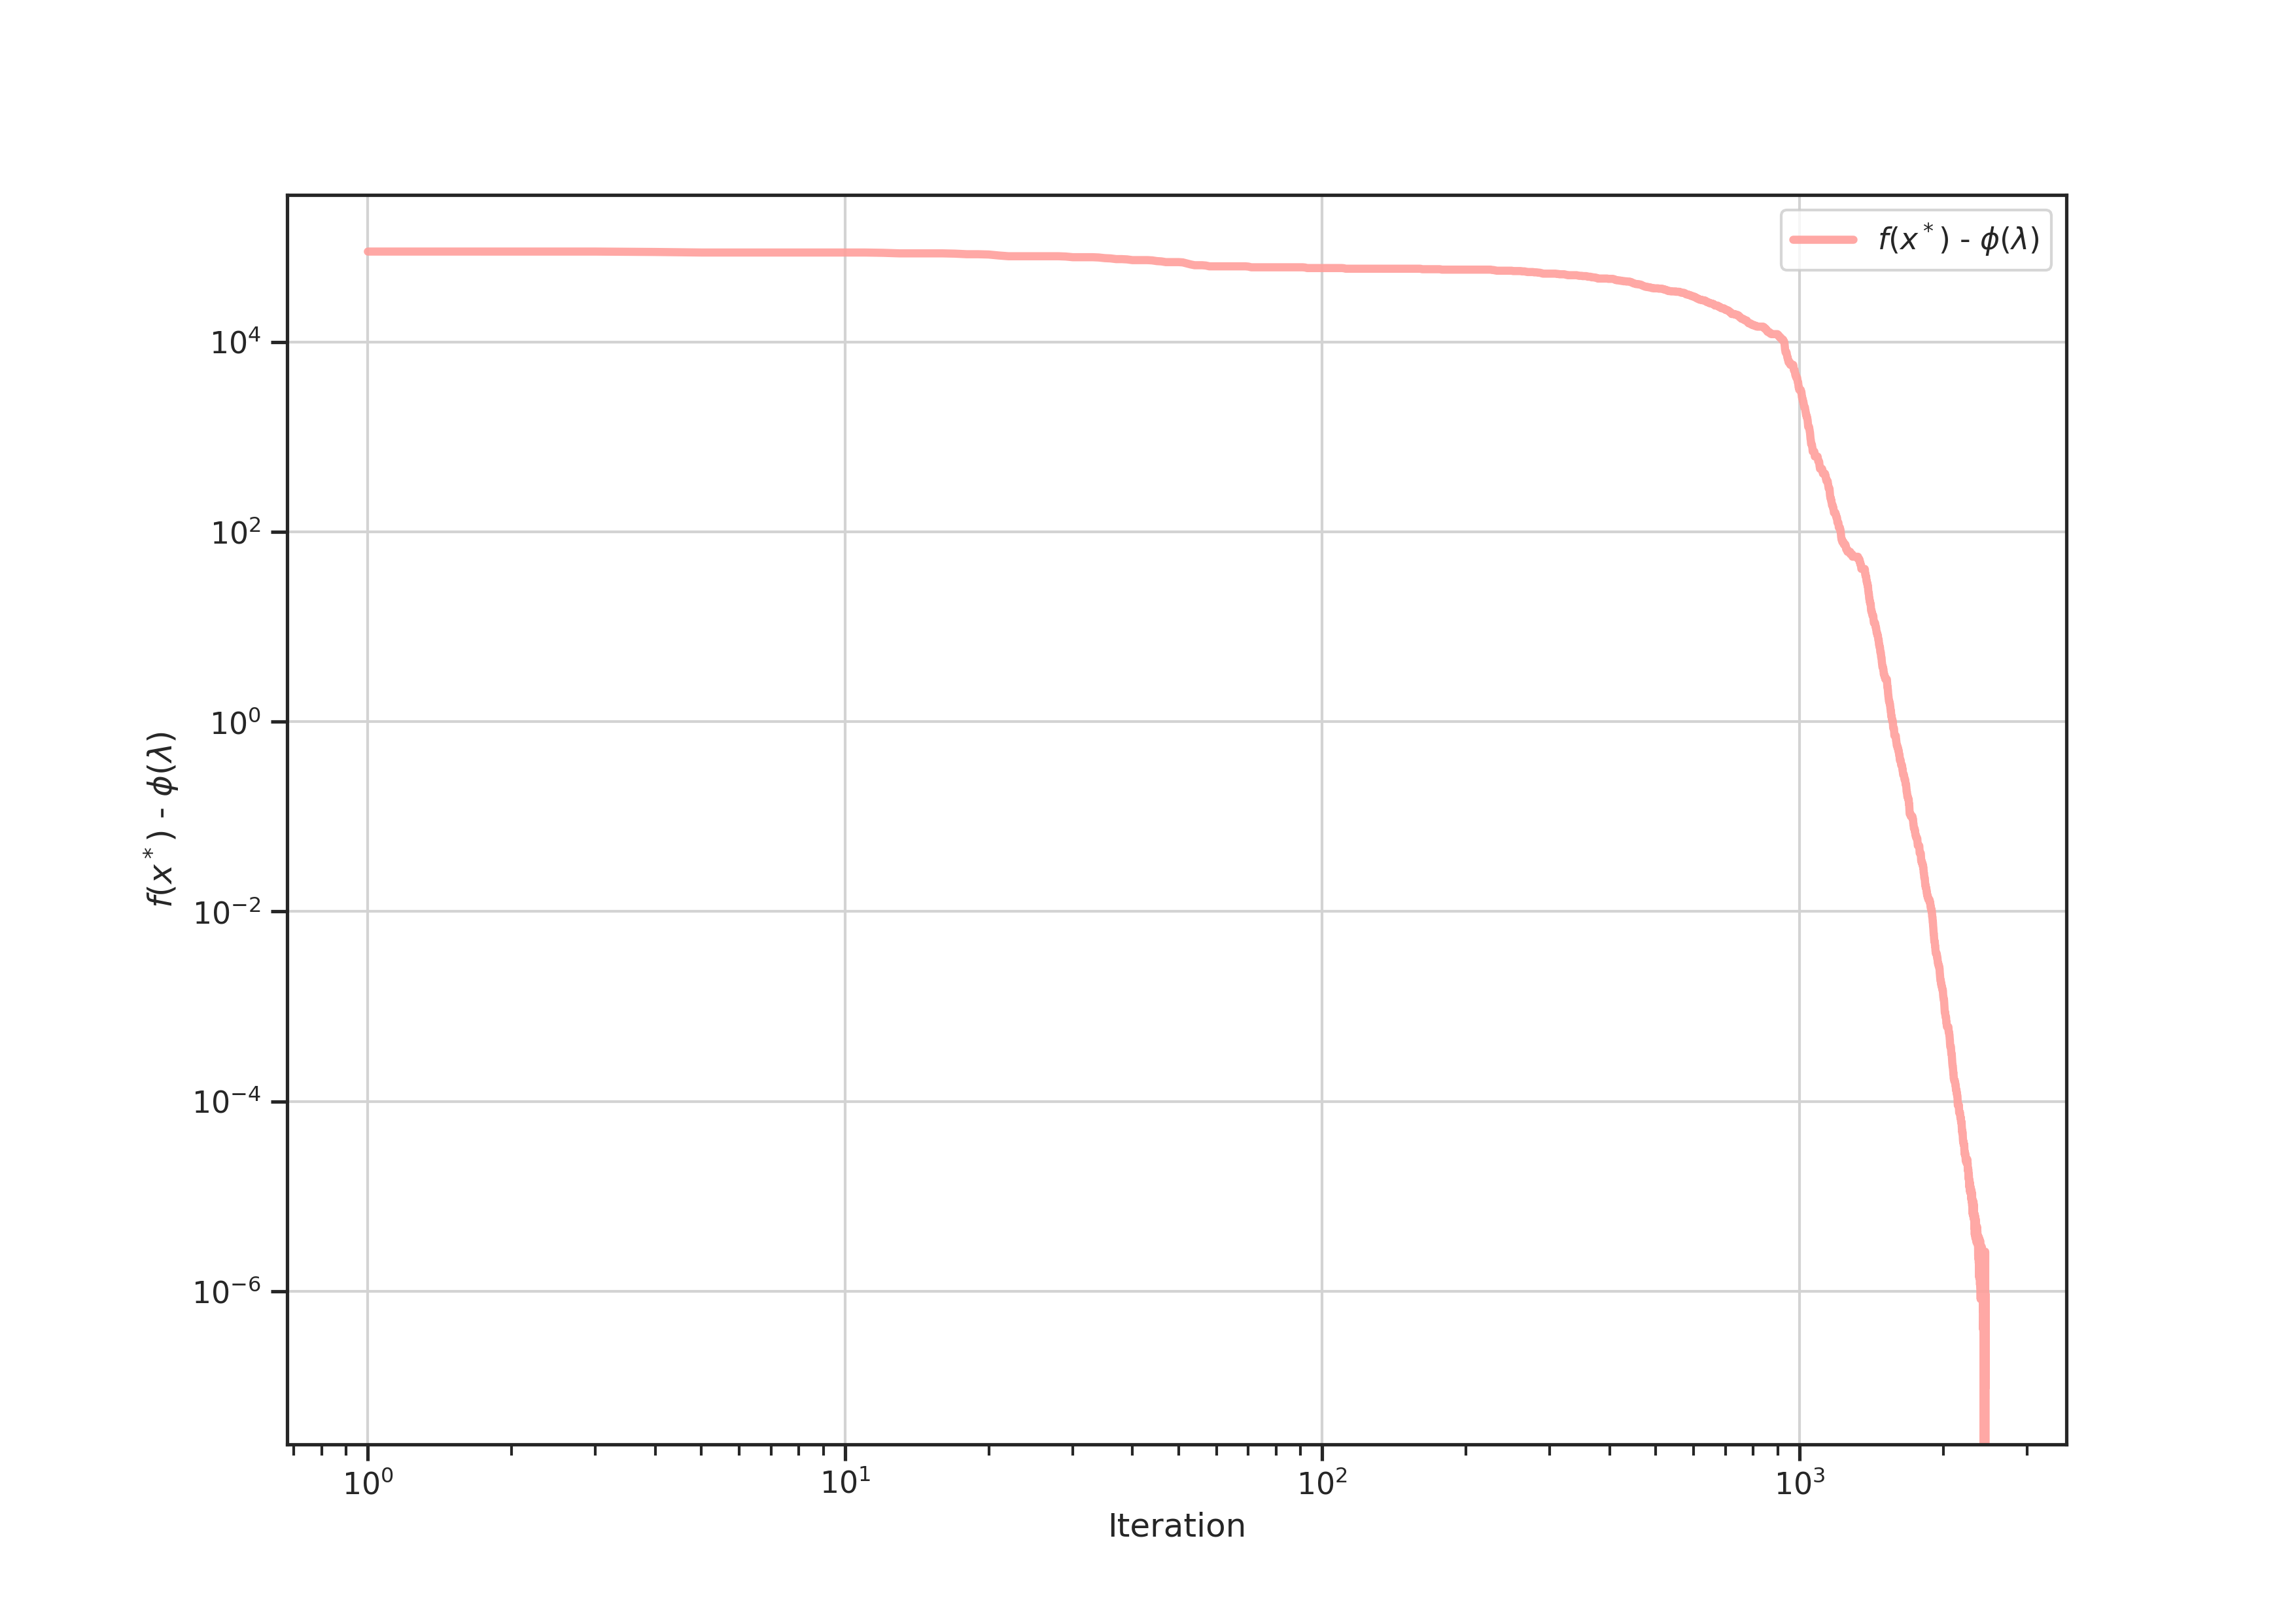
\includegraphics[scale=0.67]{pics/n=1000_K=20_gap_rule=1.png}
%   \caption{Dual gap with update rule $1$, $n=1000$ and $K=20$}
%   \label{fig:rule-1-n-1000-k-20-gap}
% \end{figure}

% \begin{figure}[H]
%   \begin{minipage}{0.49\textwidth}
%     \centering
%     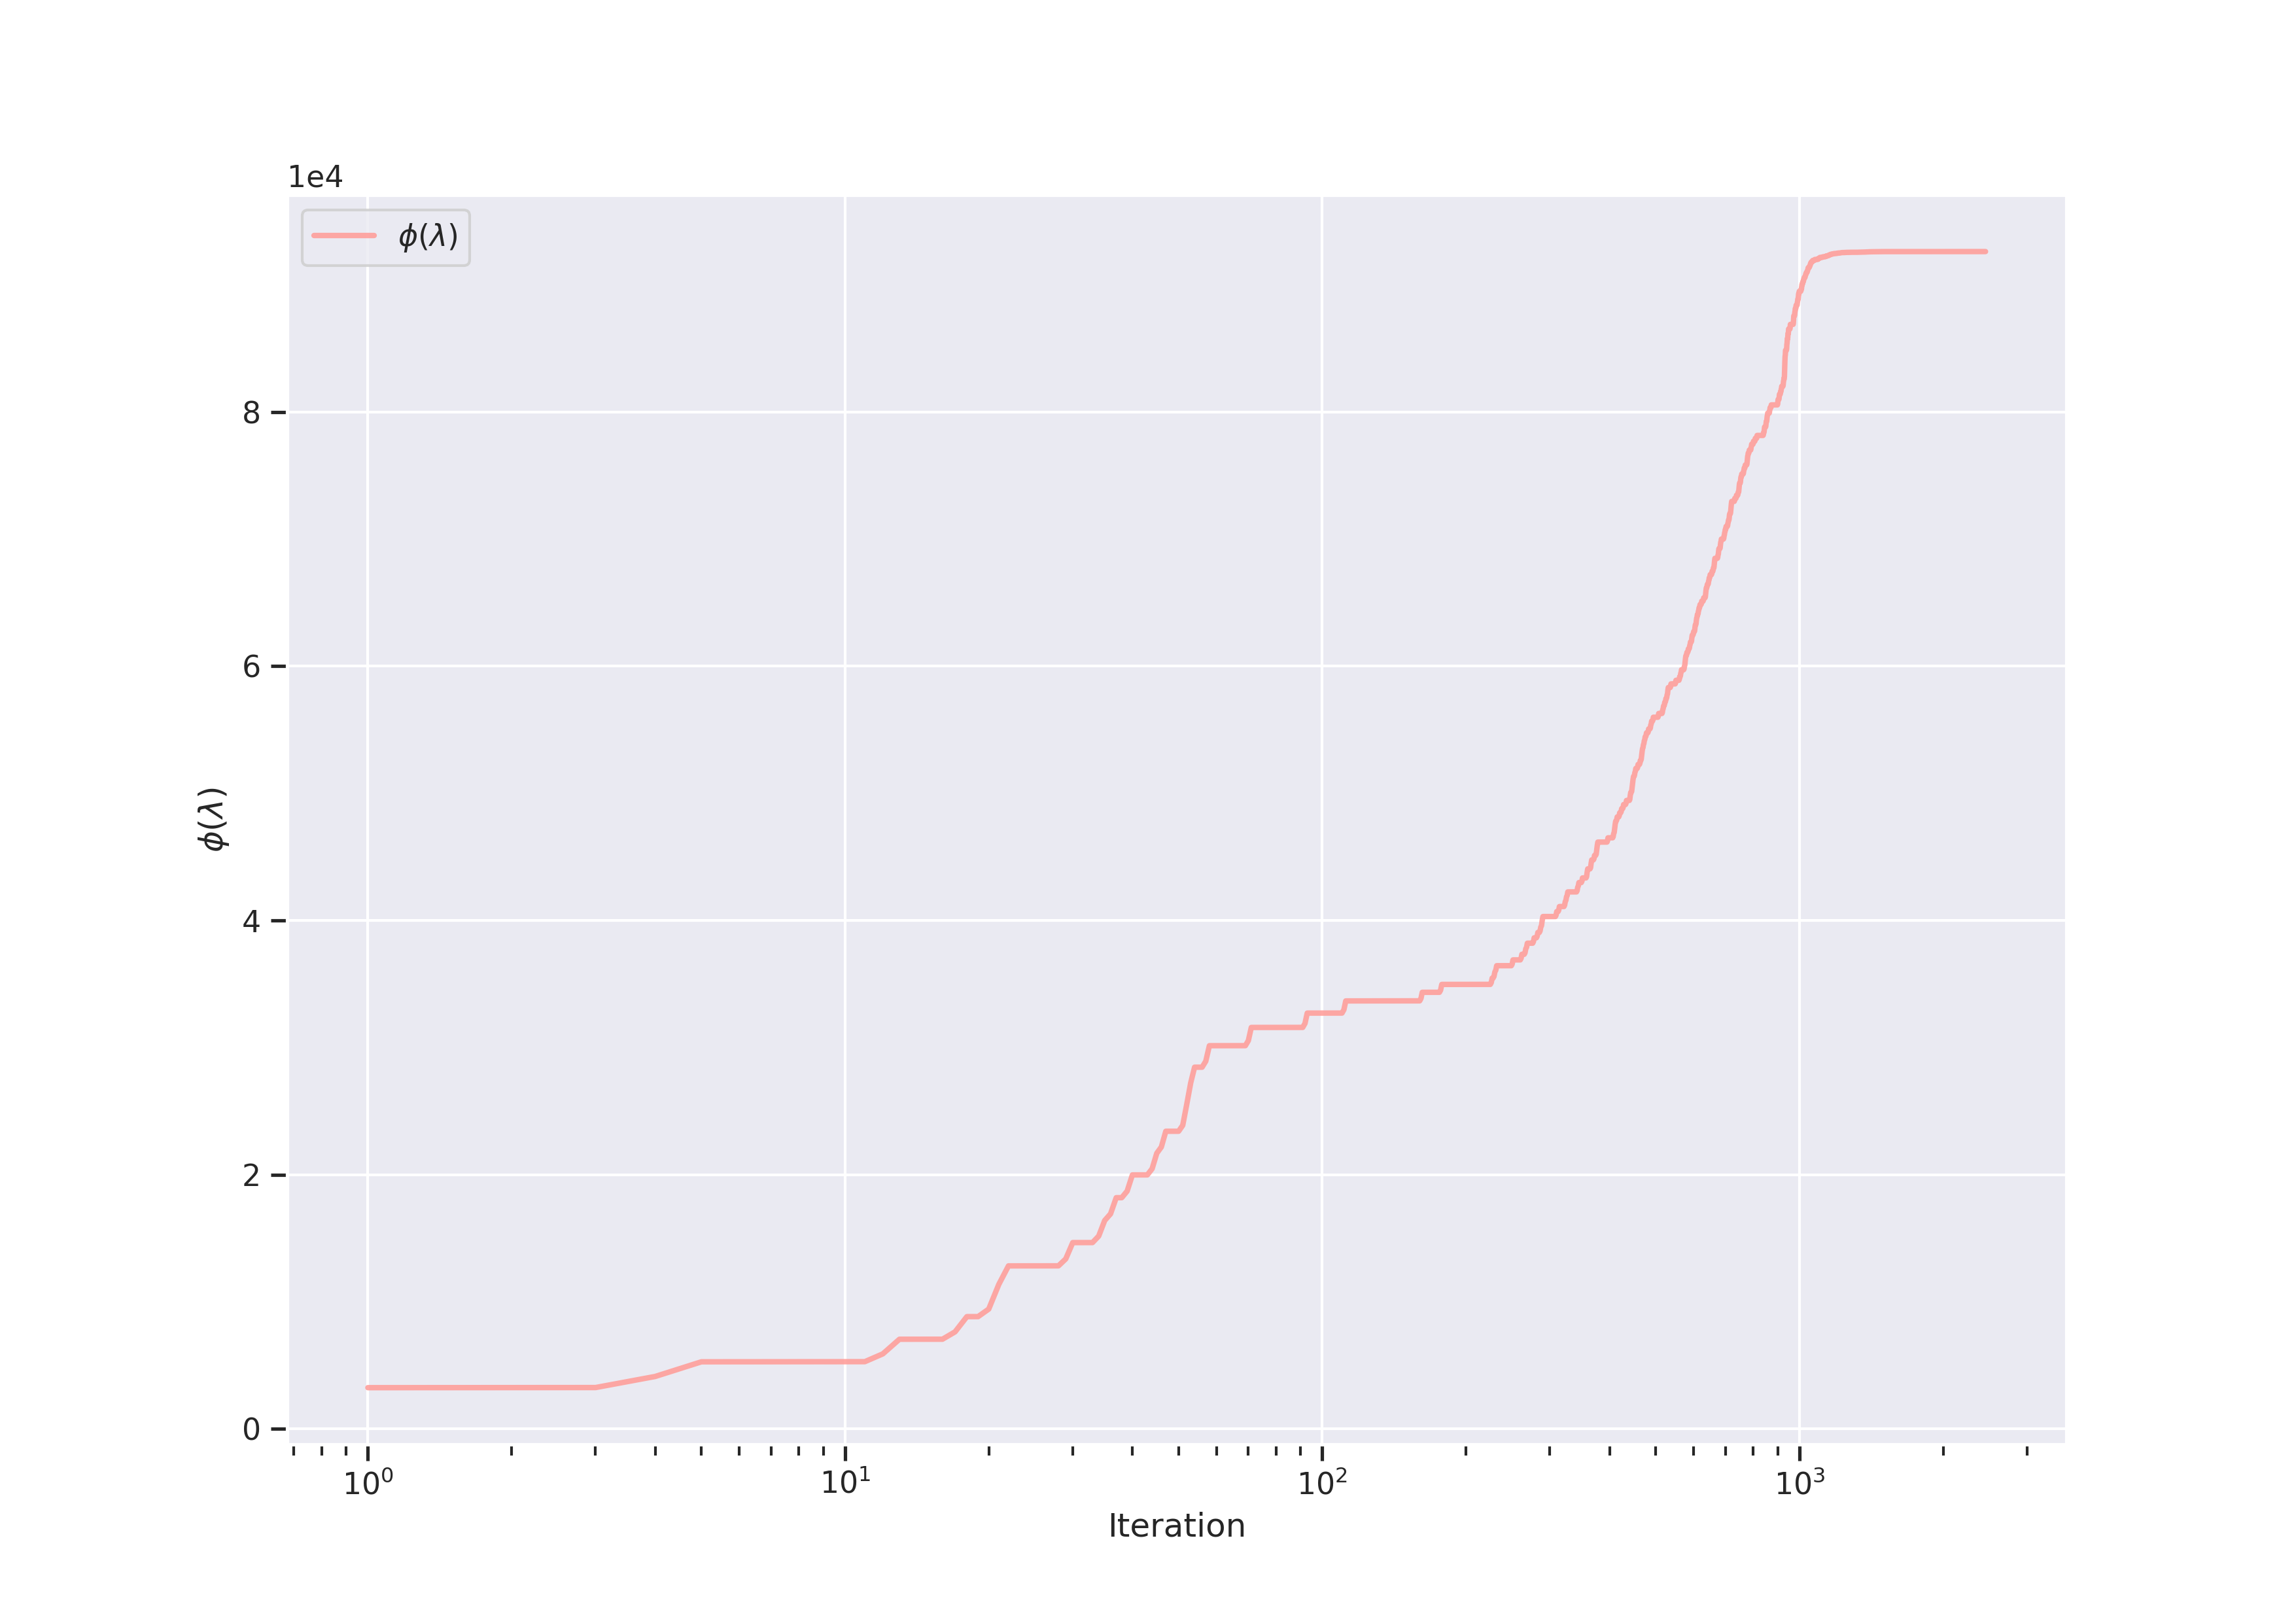
\includegraphics[scale=0.33]{pics/n=1000_K=20_dual_rule=1.png}
%     \caption{Dual value with update rule $1$, $n=1000$ and $K=20$}
%     \label{fig:rule-1-n-1000-k-20-dual}
%   \end{minipage}
%   \begin{minipage}{0.49\textwidth}
%     \centering
%     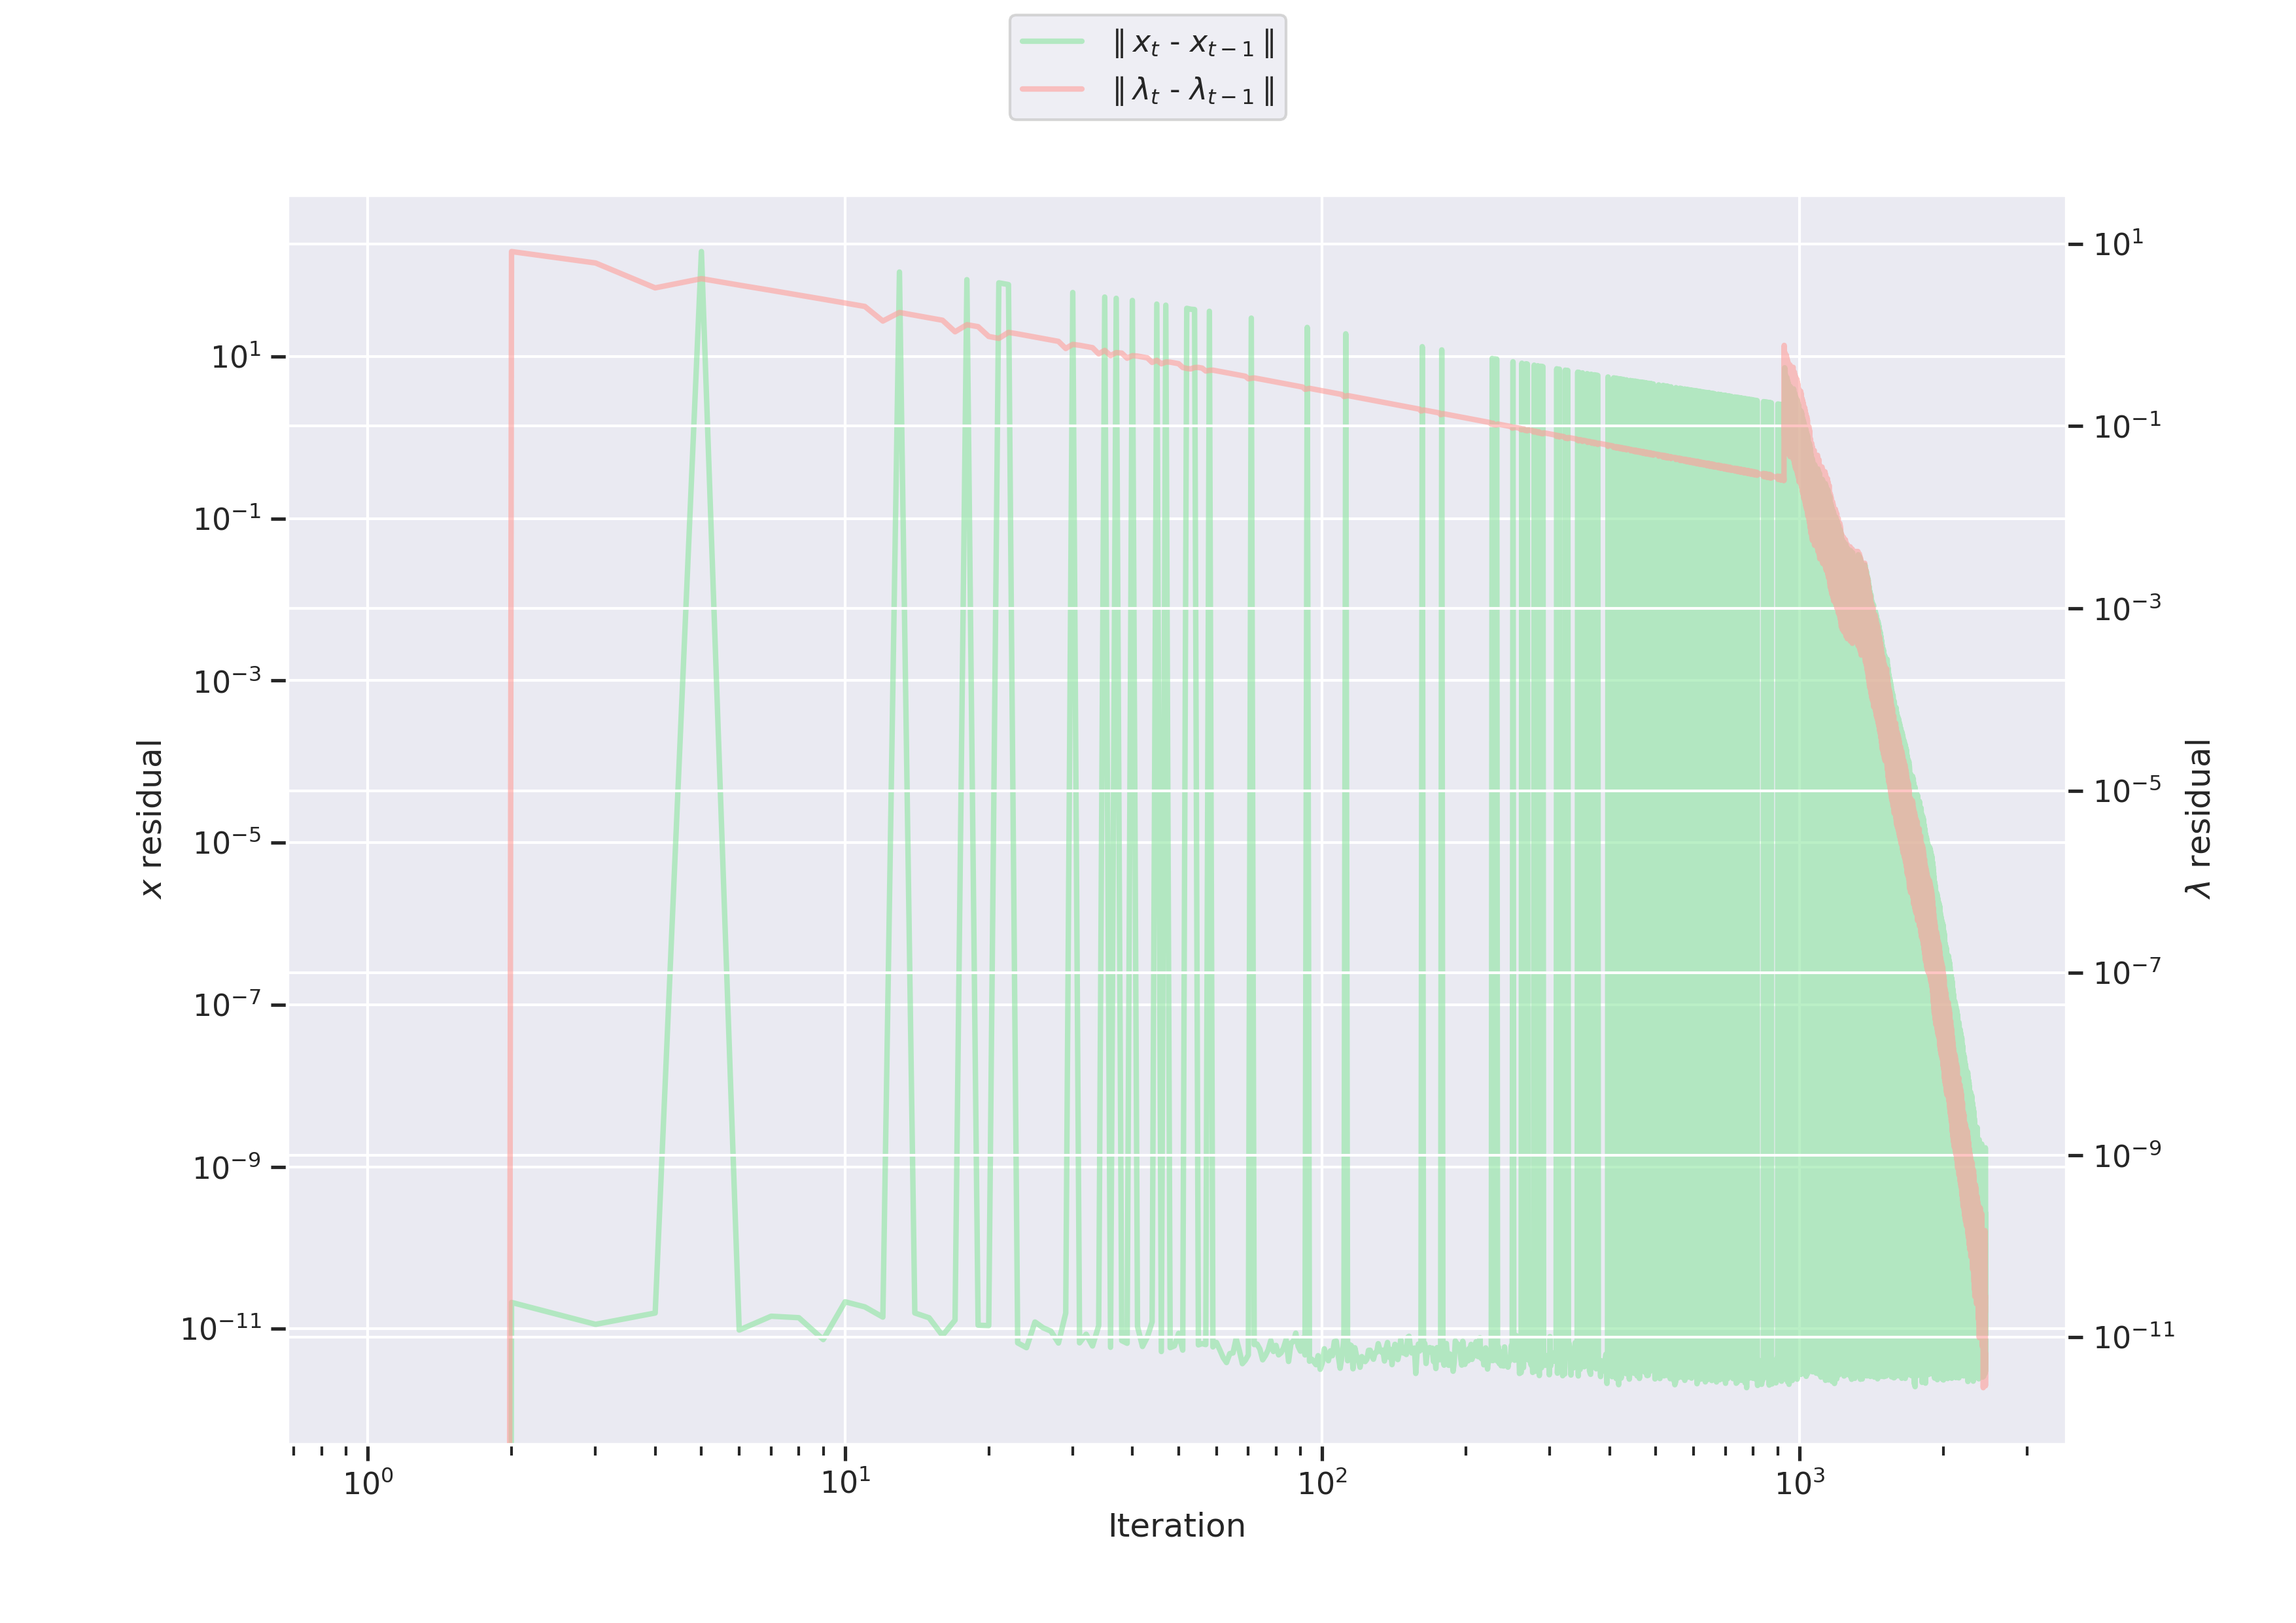
\includegraphics[scale=0.33]{pics/n=1000_K=20_lambda_rule=1.png}
%     \caption{Norms with update rule $1$, with $n=1000$ and $K=20$}
%     \label{fig:rule-1-n-1000-k-20-norm}
%   \end{minipage}  
% \end{figure}

% \vfill
% \hspace{0pt}

% \newpage

\hspace{0pt}
\vfill

% \begin{table}[H]
%   \centering
%   \resizebox{\columnwidth}{!}{%
%   \begin{tabular}{| c | c | c | c | c | c | c | c | c | c |}
%     \hline
%     $n$ & $K$ & {\itshape Update rule} & {\itshape Total iterations} & {\itshape total time (sec)} & {\itshape Best iteration} & {\itshape Best } $\phi(\lambda) - f(x^*)$ & {\itshape Best } $\psi(\lambda)$ & {\itshape Best } $\| \lambda_{t} - \lambda_{t-1} \|$ & {\itshape Best } $\| x_{t} - x_{t-1} \|$ \\
%     \hline
%     \multirow{2}{*}{$1000$} & \multirow{2}{*}{$10$} & $1$ & $2454$ & $33.1$ $s$ & $2454$ & $9.639$$e$$-08$ & $9.261$$e$$+04$ & $6.720$$e$$-12$ & $2.721$$e$$-10$ \\
%     \cline{3-10}
%      & & $3$ & $5713$ & $116.9$ $s$ & $5713$ & $1.434$$e$$-08$ & $9.261$$e$$+04$ & $1.922$$e$$-07$ & $1.041$$e$$-11$ \\
%     \hline
%   \end{tabular}
%   }%
% \end{table}

\begin{minipage}{.7\textwidth}
  \begin{figure}[H]
    \centering
    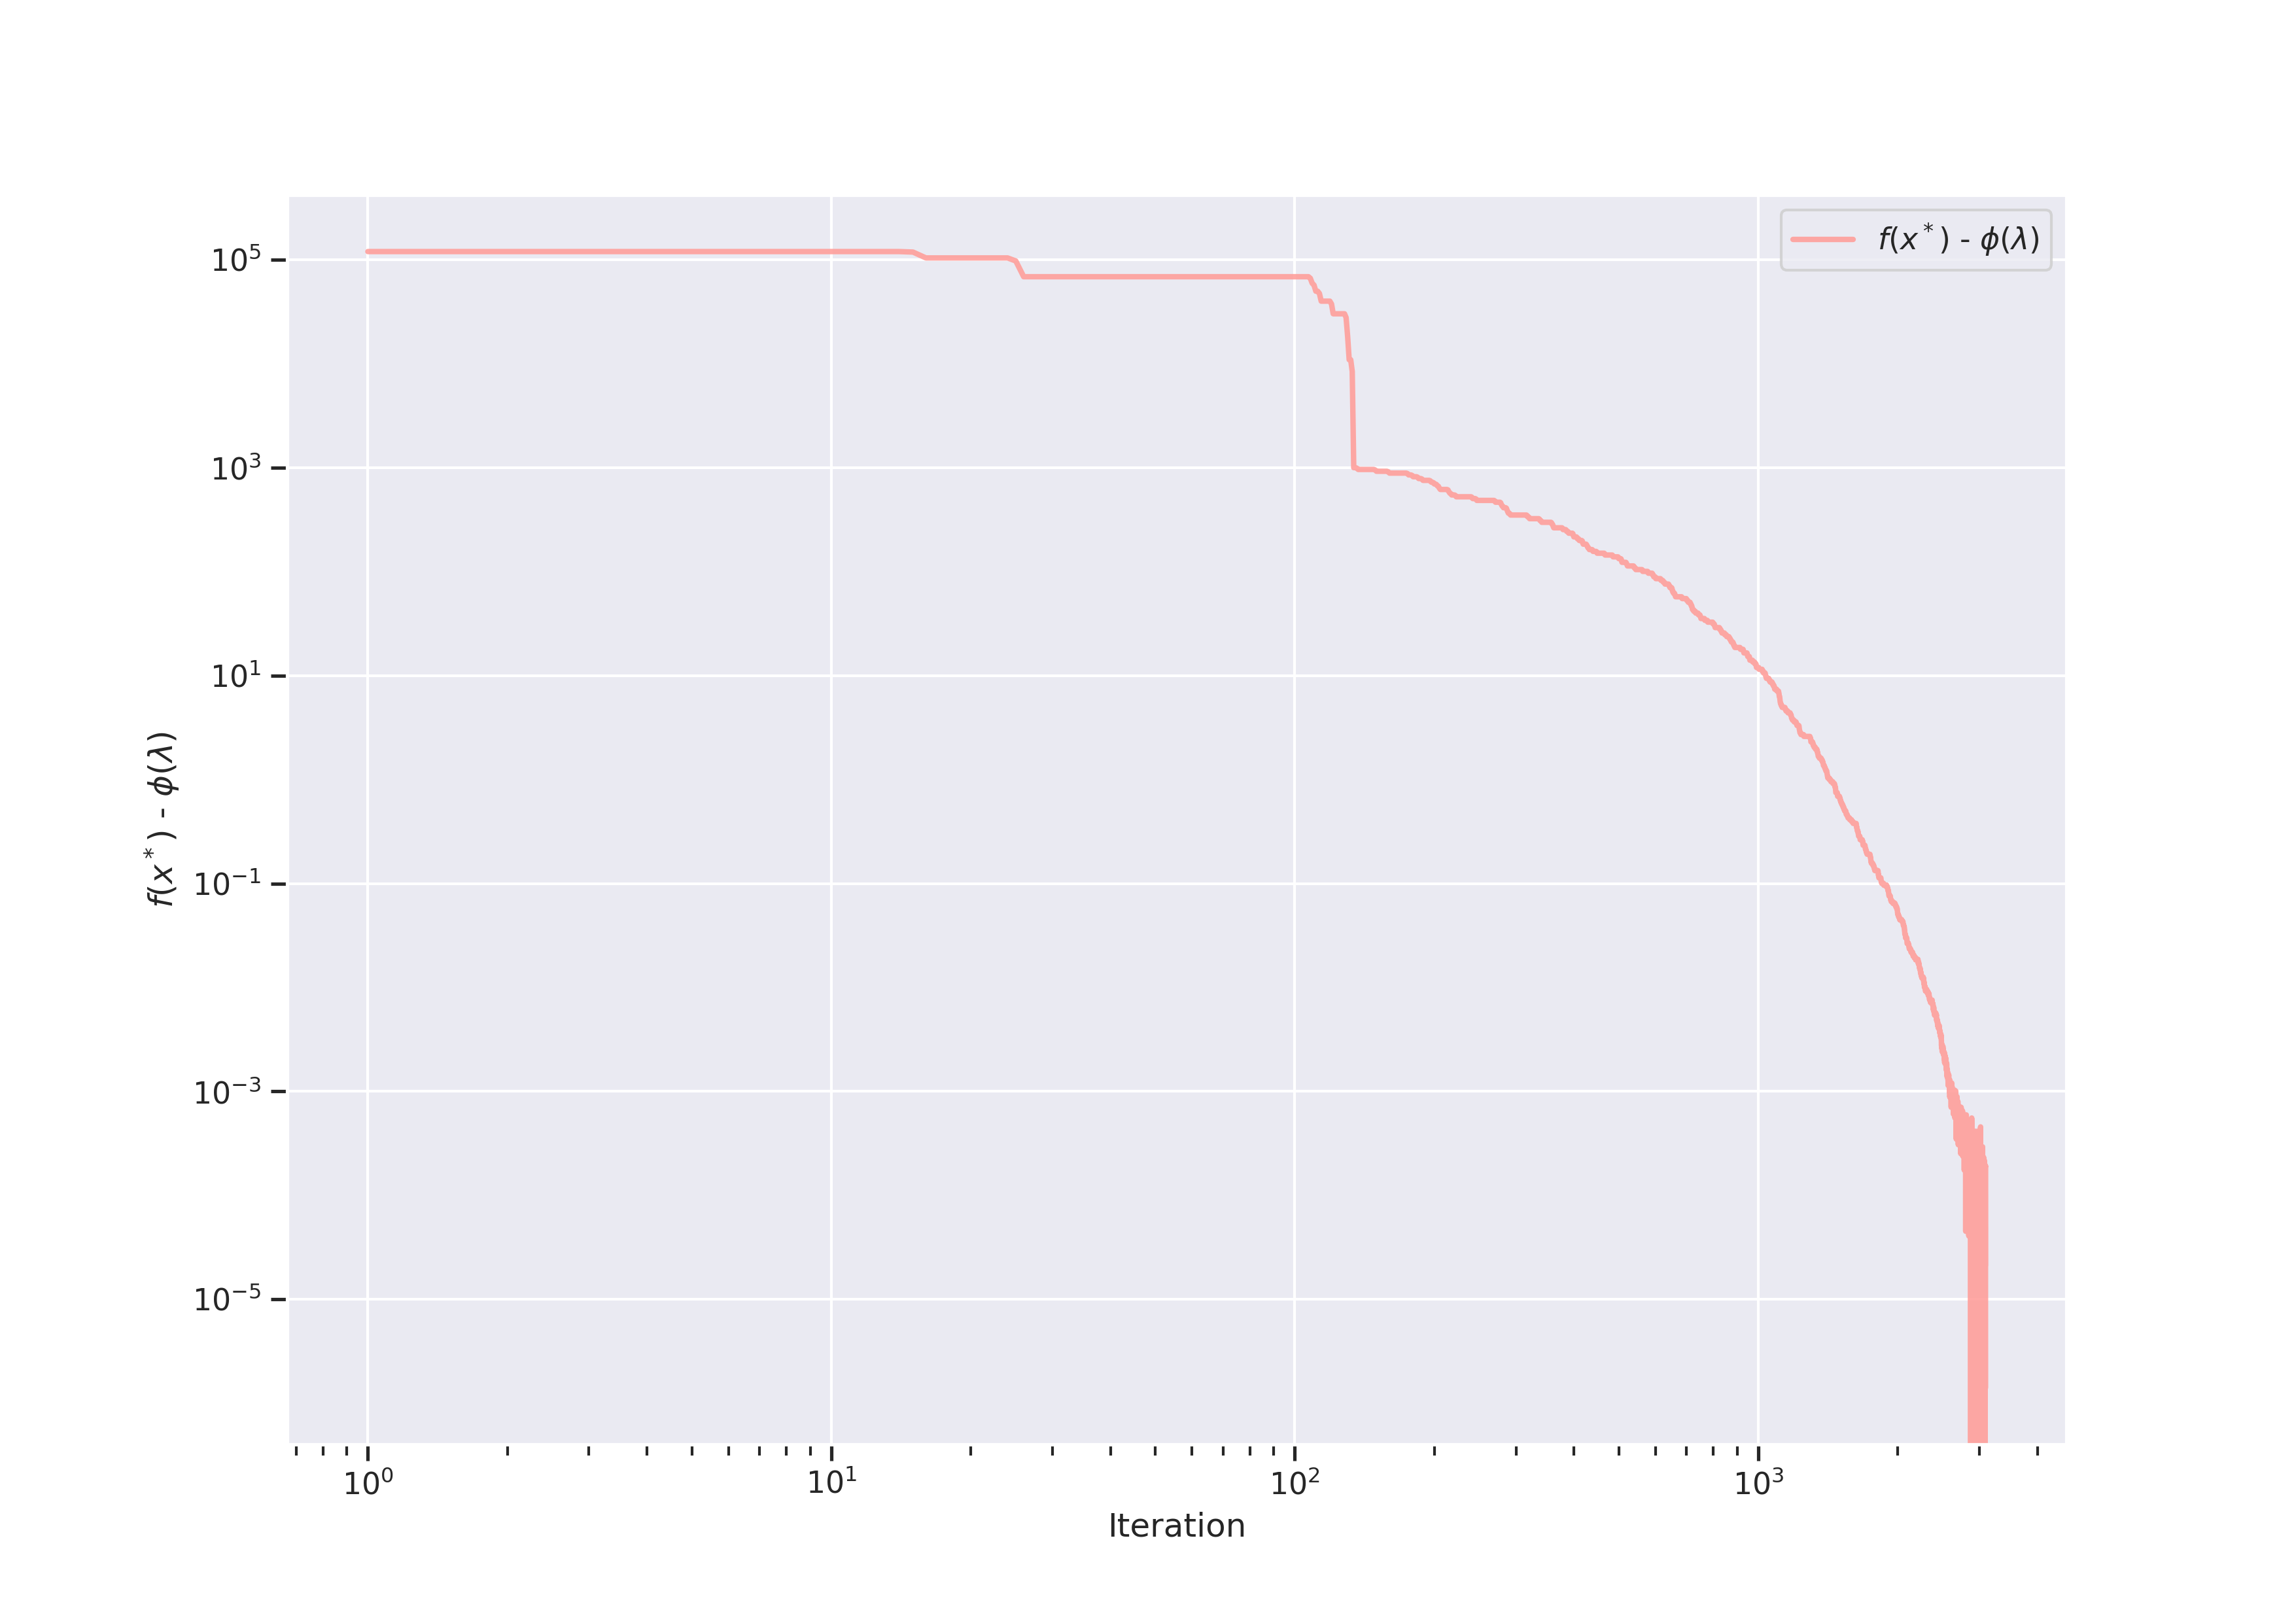
\includegraphics[scale=0.5]{pics/n=5000_K=10_gap_rule=1.png}
    \caption{Dual gap with update rule $1$, $n=5000$ and $K=10$}
    \label{fig:rule-1-n-5000-k-10-gap}
  \end{figure}
\end{minipage}
\begin{minipage}{.3\textwidth}
  \begin{table}[H]
    \centering
    \resizebox{\columnwidth}{!}{%
    \begin{tabular}{| c | c |}
      \hline
      {\itshape Total iterations} & $3092$ \\
      \hline
      {\itshape total time (sec)} & $665.3 \, s$ \\
      \hline 
      {\itshape Best } $\phi(\lambda) - f(x^*)$ & $1.414e$$-$$06$ \\
      \hline
      {\itshape Best iteration} & $3092$ \\
      \hline
      {\itshape Best } $\psi(\lambda)$ & $1.202e$$+$$05$ \\
      \hline
      {\itshape Best } $\| \lambda_{t} - \lambda_{t-1} \|$ & $2.586e$$-$$08$ \\
      \hline
      {\itshape Best } $\| x_{t} - x_{t-1} \|$ & $5.190e$$-$$11$ \\
      \hline
    \end{tabular}
    }%
    \caption{\centering Sum up table for $n=5000$, $K=10$ and rule $1$}
    \label{tab:n-5000-K-10-rule-1}
  \end{table}
\end{minipage}

\vspace{1em}

\begin{changemargin}{3.5cm}{3.5cm}
  Let's look in depth now at the results using the update rule $1$, on a problem of dimension $n=5000$ and $K=10$. As we can see from above, there are different considerations to do.
  First of all we can see how we are capable of reaching the desired dual gap, in the order of $10^{-6}$.\\
  To reach the optimal solution, the experimentation took the following approach:
  \begin{itemize}
    \item First of all, we created the problem structures ($Q$, $I_K$, $A$) and stored them in a \textit{.mat} file;
    \item Then, we used the structures created on \texttt{YALMIP} to compute the optimal $p^*$ of the primal problem;
    \item Obtained the solution, this was imported in the \textit{Julia} code and used to compute the dual gap;
  \end{itemize}
  In order to get the best out from our solver, we tried different times by changing the hyperparameters. For the update rule $1$, we decided to focus on the {\itshape Nonsummable diminishing} 
  stepsize rule and then on the {\itshape Polyak} stepsize rule.\\
  We discovered that using \textit{Polyak} stepsize is necessary in the tail of our convergence, in order to avoid divergence due to big steps.\\
  Instead, in the starting part of our algorithm, an optimal value we found for the only hyperparameter $\alpha$ is $0.3$. In this way, we perform neither too big steps nor too small steps, 
  reaching the optimal solution in a fair amount of iterations.\\
  Changing also slightly the hyperparameter $\alpha$ results in an uncontrolled behavior (for example if we put too small $\alpha$) or in the other case in a too slow behavior (when we give $\alpha$
  an high value).\\
  We tried also using \textit{Polyak} stepsize from iteration $0$, but we noticed that convergence was slow and we could improve it by using the above approach.\\
  In addition, we tried to use the classical {\itshape Square summable but not summable} rule, which give us a very slow convergence rate, even changing the value of $\alpha$. Using this stepsize 
  rule requires a lot of time and iterations, but from theory we know that even if slow the convergence is guaranteed.
\end{changemargin}

\vfill
\hspace{0pt}

\newpage

\vfill
\hspace{0pt}

\begin{minipage}{.7\textwidth}
  \begin{figure}[H]
    \centering
    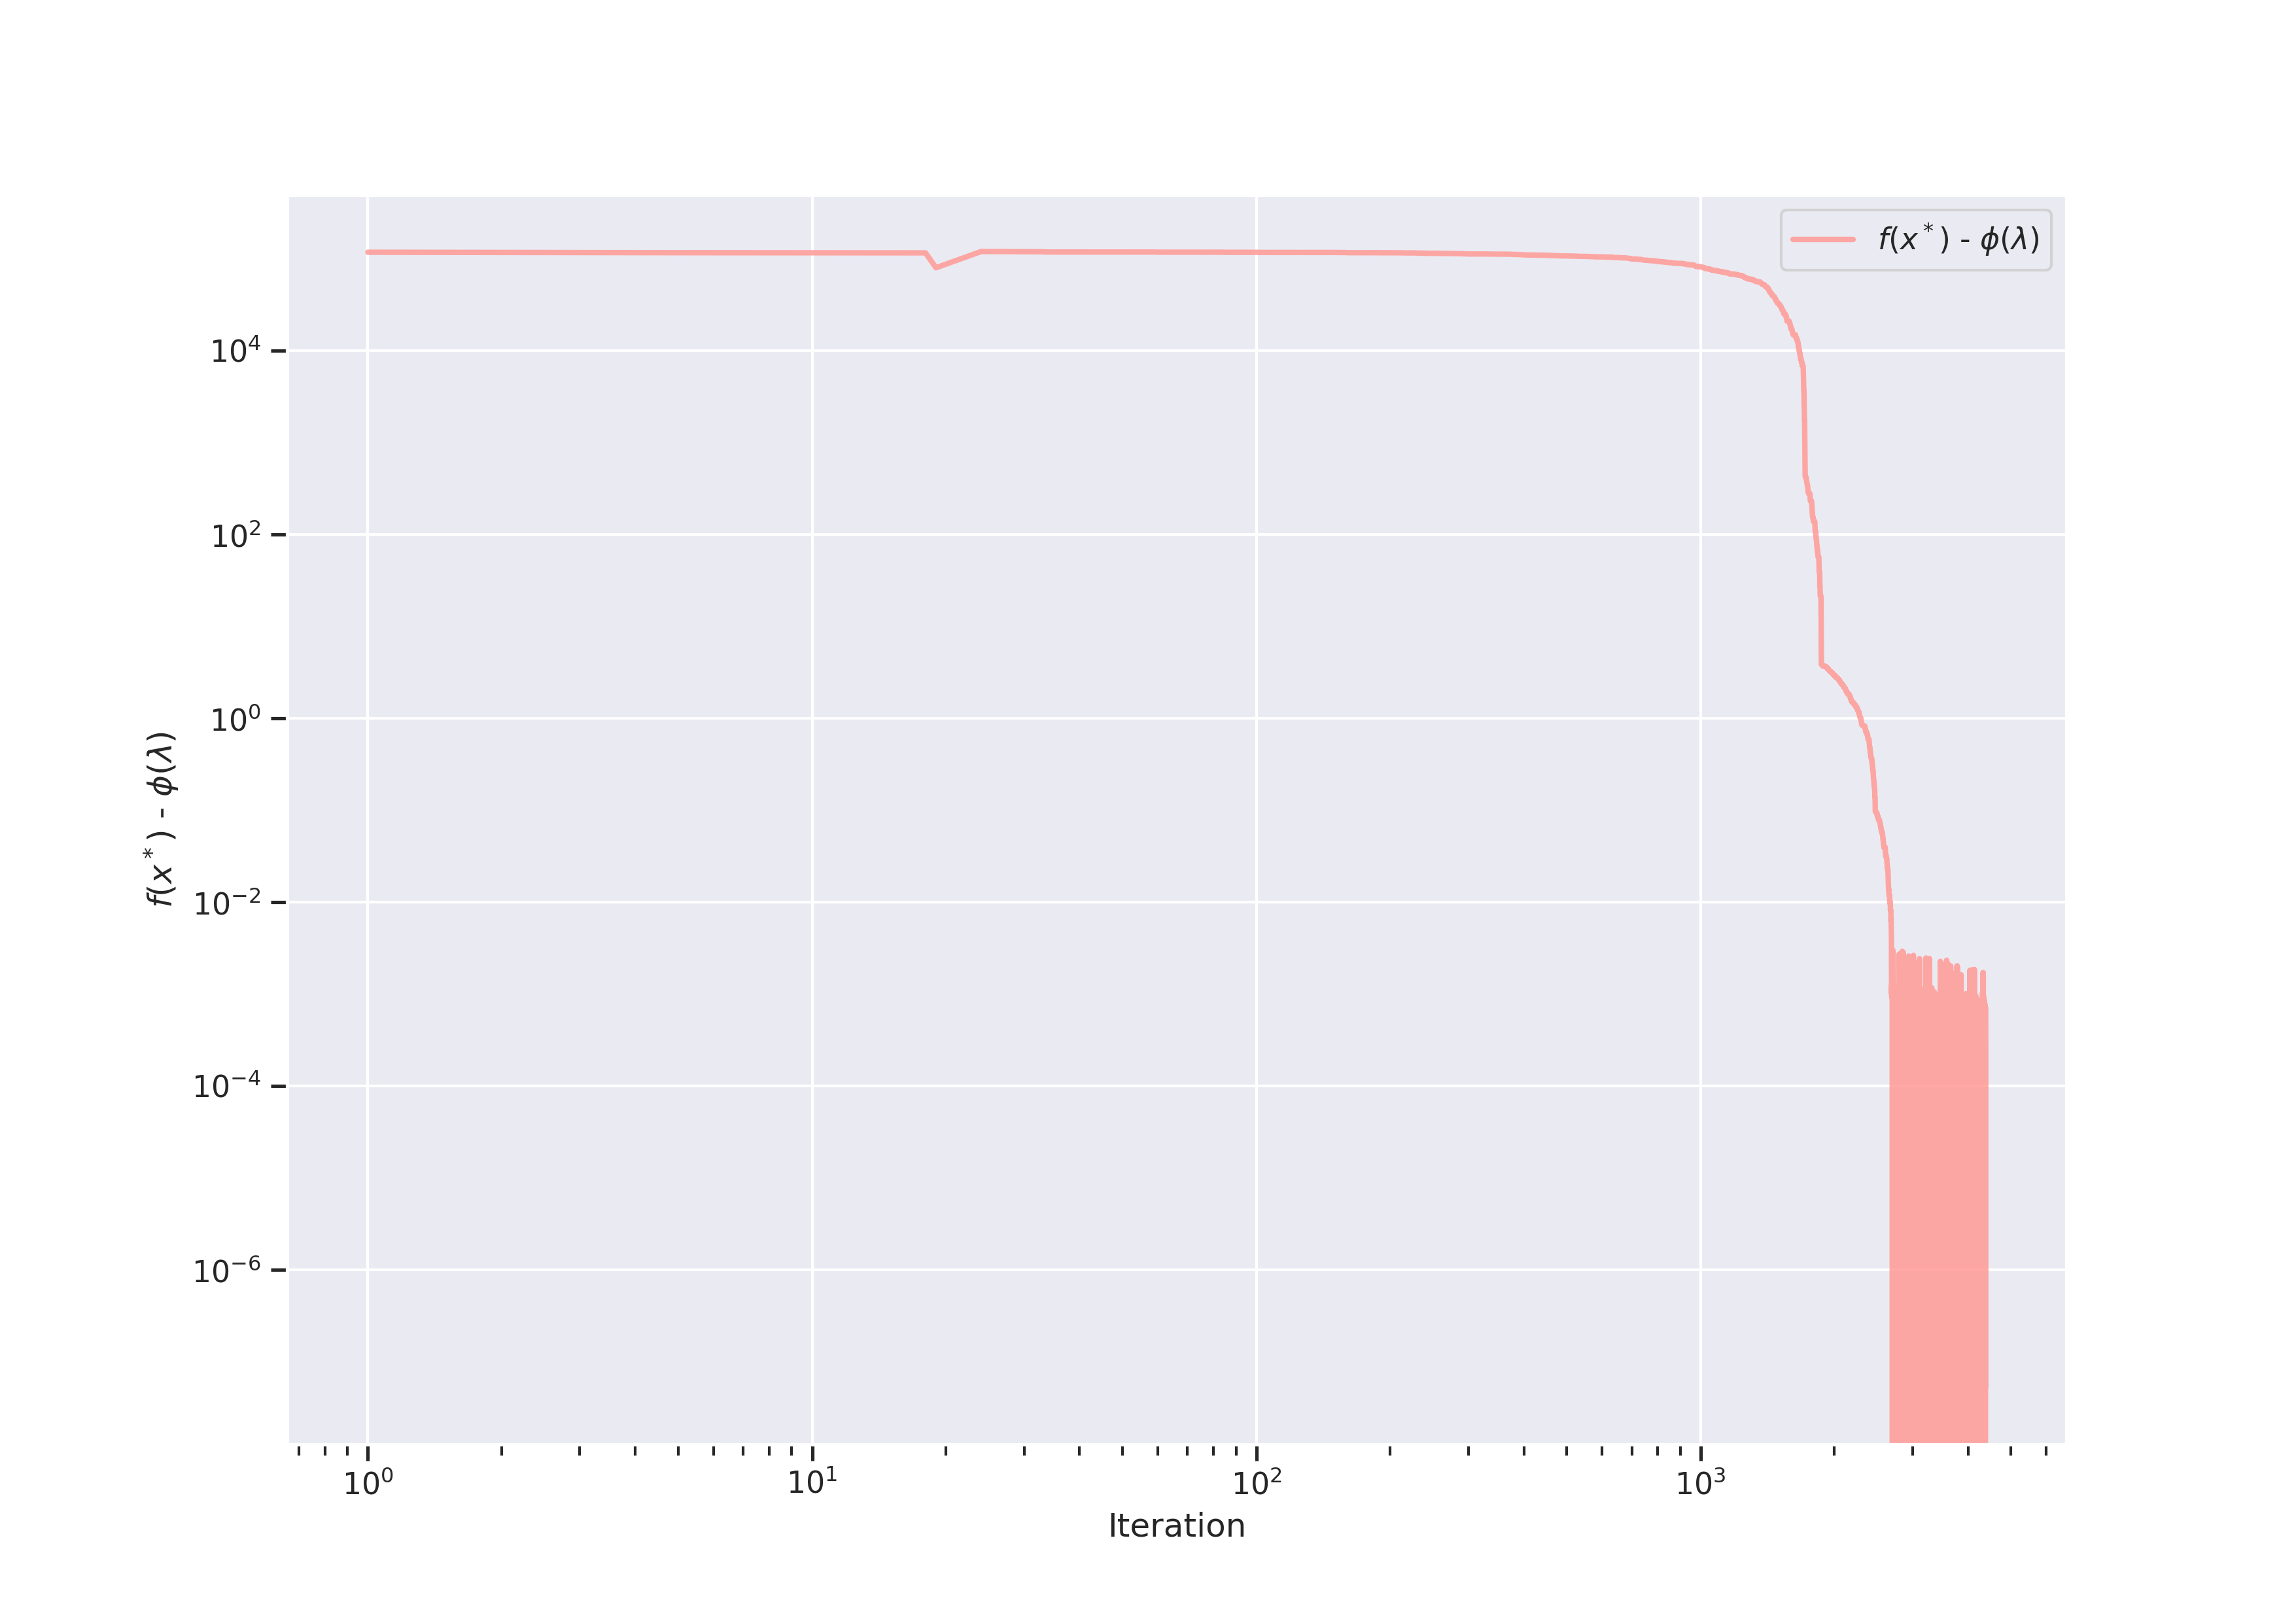
\includegraphics[scale=0.5]{pics/n=5000_K=10_gap_rule=3.png}
    \caption{Dual gap with update rule $3$, $n=5000$ and $K=10$}
    \label{fig:rule-3-n-5000-k-10-gap}
  \end{figure}
\end{minipage}
\begin{minipage}{.3\textwidth}
  \begin{table}[H]
    \centering
    \resizebox{\columnwidth}{!}{%
    \begin{tabular}{| c | c |}
      \hline
      {\itshape Total iterations} & $4379$ \\
      \hline
      {\itshape total time (sec)} & $952.5 \, s$ \\
      \hline 
      {\itshape Best } $\phi(\lambda) - f(x^*)$ & $5.243e$$-$$08$ \\
      \hline
      {\itshape Best iteration} & $4379$ \\
      \hline
      {\itshape Best } $\psi(\lambda)$ & $1.202e$$+$$05$ \\
      \hline
      {\itshape Best } $\| \lambda_{t} - \lambda_{t-1} \|$ & $1.471e$$-$$09$ \\
      \hline
      {\itshape Best } $\| x_{t} - x_{t-1} \|$ & $4.153e$$-$$05$ \\
      \hline
    \end{tabular}
    }%
    \caption{\centering Sum up table for $n=5000$, $K=10$ and rule $3$}
    \label{tab:n-5000-K-10-rule-3}
  \end{table}
\end{minipage}

\vspace{1cm}

\begin{changemargin}{3.5cm}{3.5cm}
  In this other case, we approach the same problem dimension but this time using the update rule $3$. This update rule has a totally different behavior w.r.t. the above one.\\ 
  We tried using both the summable and nonsummable rules, but changing the value of $\alpha$ in this case does not led us to a good optimization. Indeed, we noticed how the solution can diverge 
  into high negative gaps or remain fixed at some high gap value, showing no improvement for a lot of iterations (in the order of $10^3$).\\
  We thought that this behavior comes from the use of the "regularizer" matrix $H_t$, which is used at the denominator to scale the step at each iteration based on the accumulated gradient. To deal with 
  this problem, we decided to change the value of the hyperparameter $\delta$, added to the matrix $H_t$. We tried scaling it both in bigger values ($> 1$) and smaller values ($< 1$), founding in the 
  end the value of $\delta = 10^{-16}$. Even changing $\delta$ and $\alpha$ brings no improvement when using this kind of rule.\\
  Analyzing the values, the problem is indeed in using a $< 1$ stepsize and the scaling matrix $H_t$, which scale too much the update part and consequently do not update $\lambda$. To overcome 
  this situation, we switched to the {\itshape constant step rule}, using a possible high fixed value of $h$ to perform big steps.\\
  Also in this situation, we did different experimentation using possible values of $h$.\\
  Similar as before, keeping an high value of $h$ in the tail is not the best approach, since we risk of diverging from the optimal gap and as a consequence never reach smaller values.\\
  The solution to this problem was to modify the value of $h$ iteratively during the optimization. Having the optimal $p^*$ at our disposal, we can use the dual gap computed at each step to decrease the 
  magnitude of $h$ as soon as we approach the optimal gap.\\
  Using this pattern, we used the following values of $h$:
  \[ \left[ 200, 25, 5, 2, 10^{-2}, 10^{-3} \right] \]
\end{changemargin}

\vfill
\hspace{0pt}

% \begin{figure}[H]
%   \begin{minipage}{0.49\textwidth}
%     \centering
%     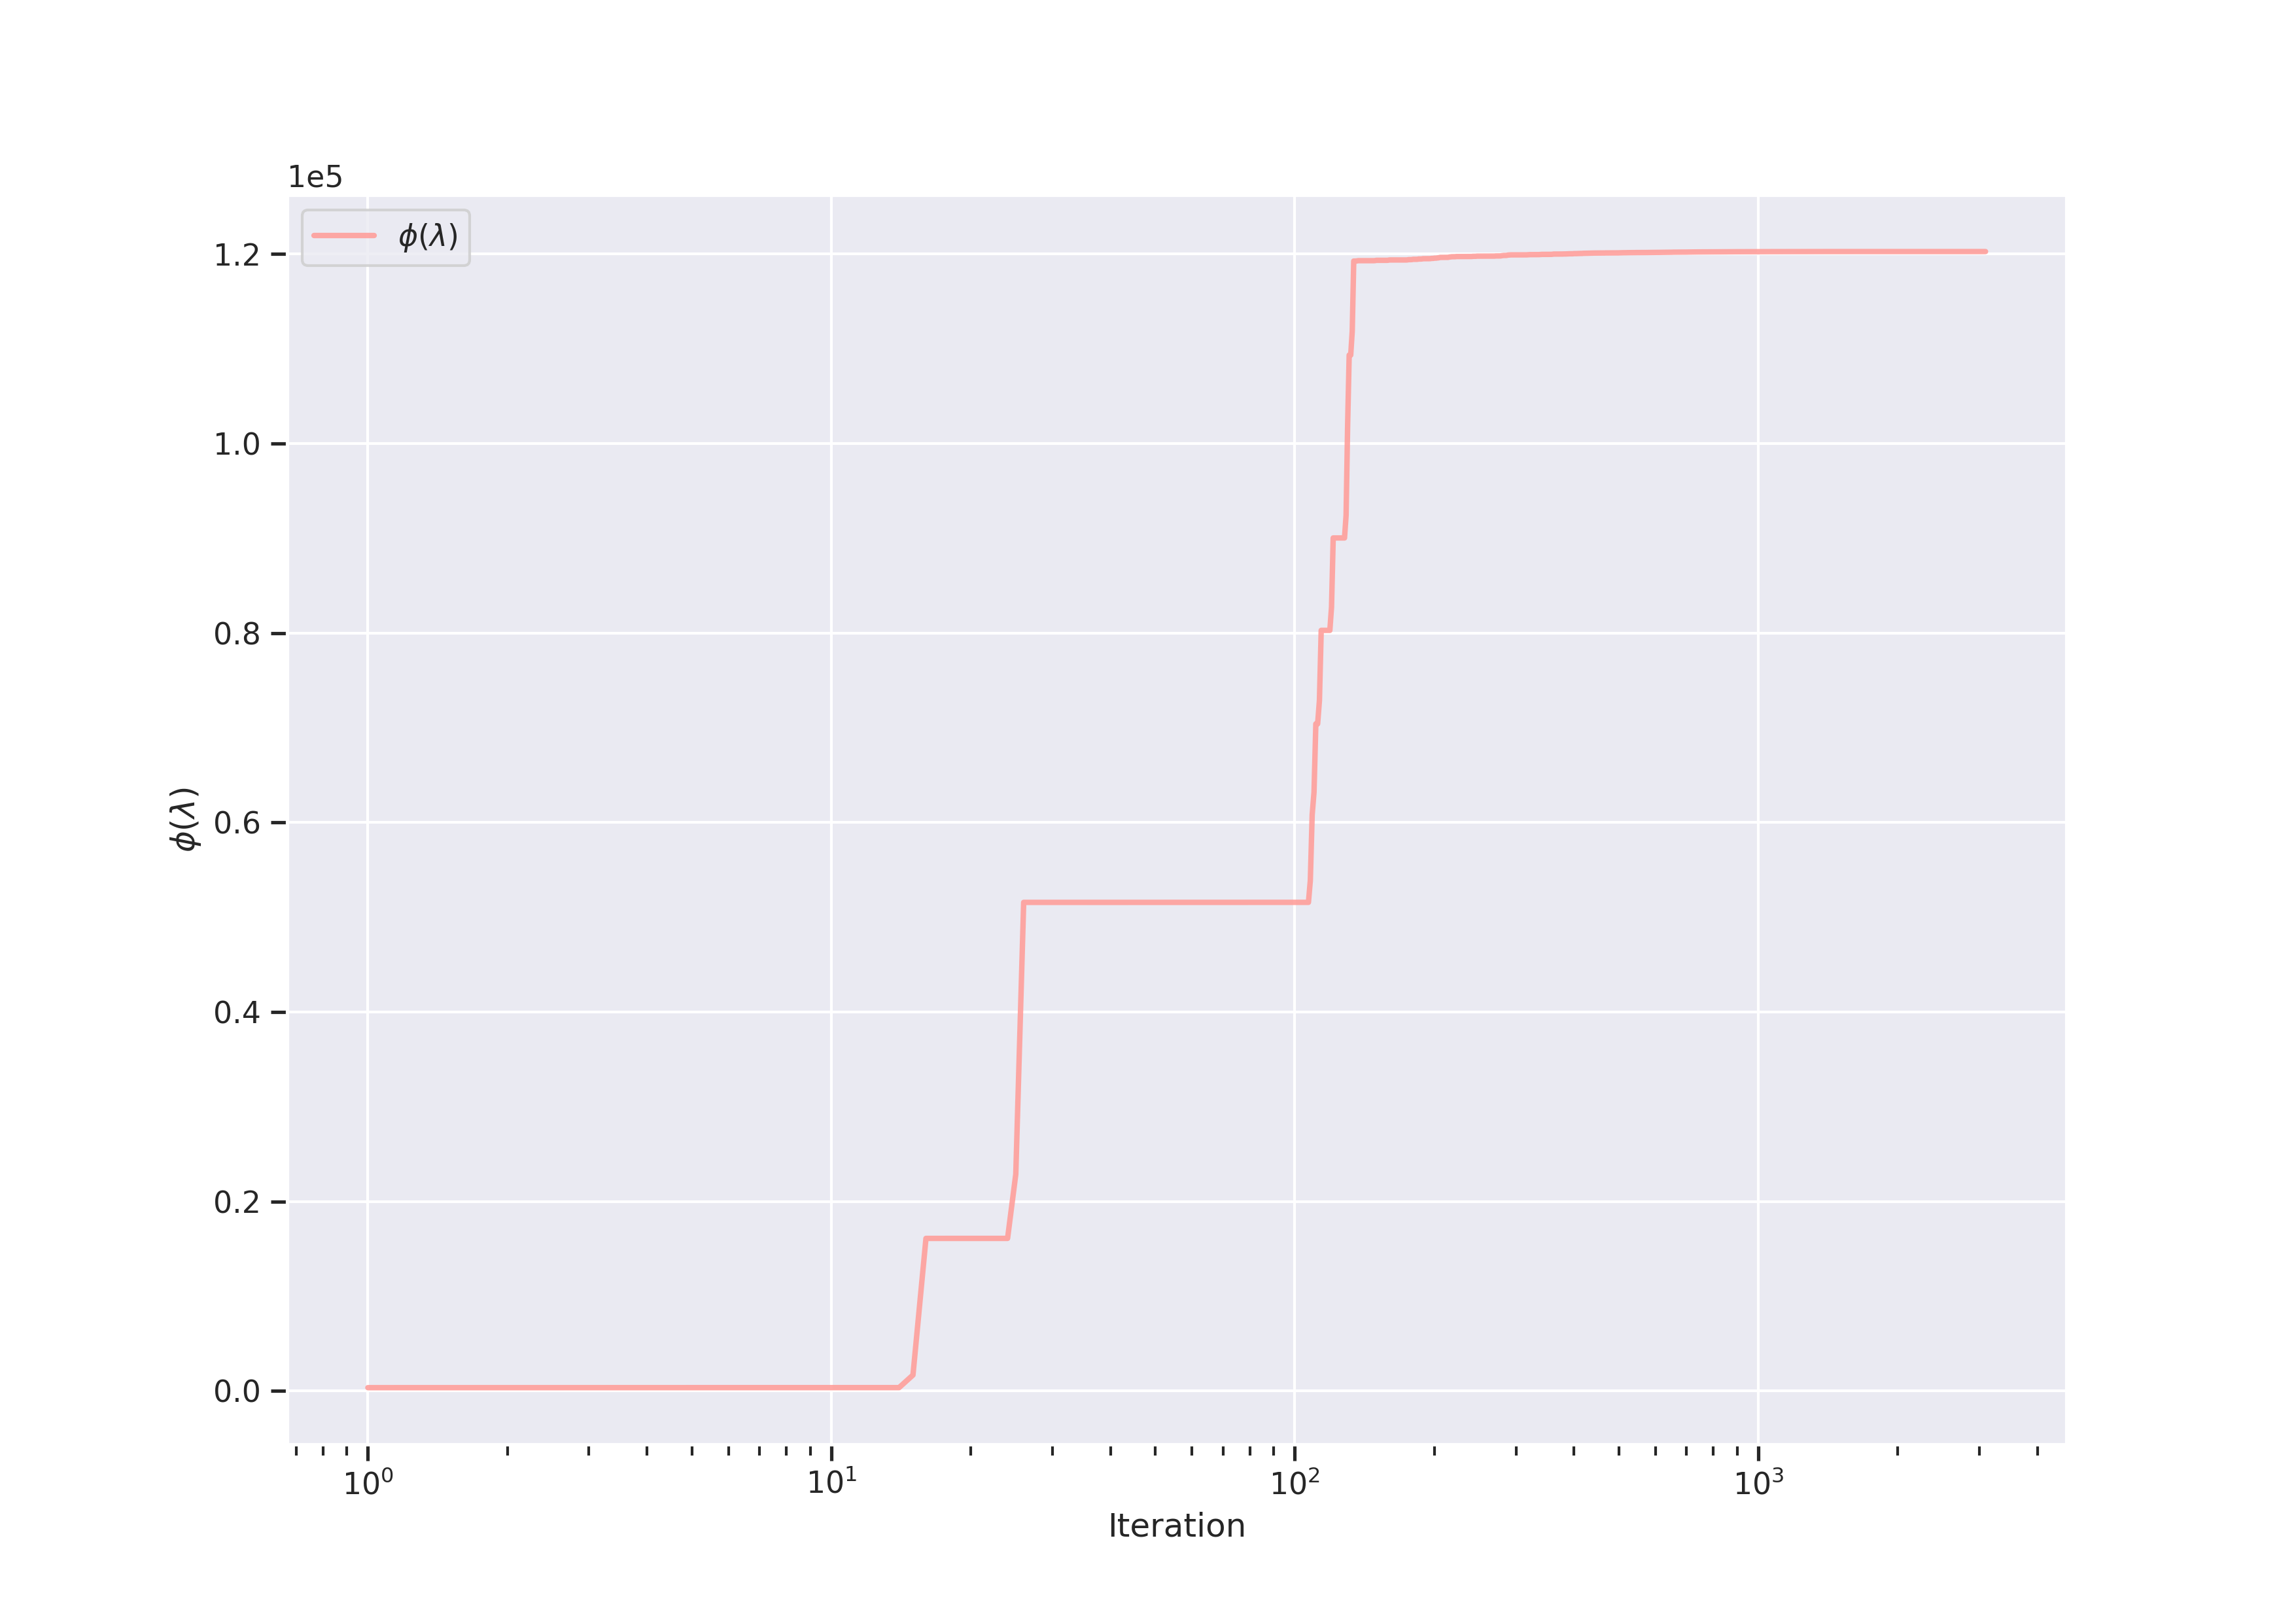
\includegraphics[scale=0.33]{pics/n=5000_K=10_dual_rule=1.png}
%     \caption{Dual value with update rule $1$, $n=5000$ and $K=10$}
%     \label{fig:rule-1-n-5000-k-10-dual}
%   \end{minipage}
%   \begin{minipage}{0.49\textwidth}
%     \centering
%     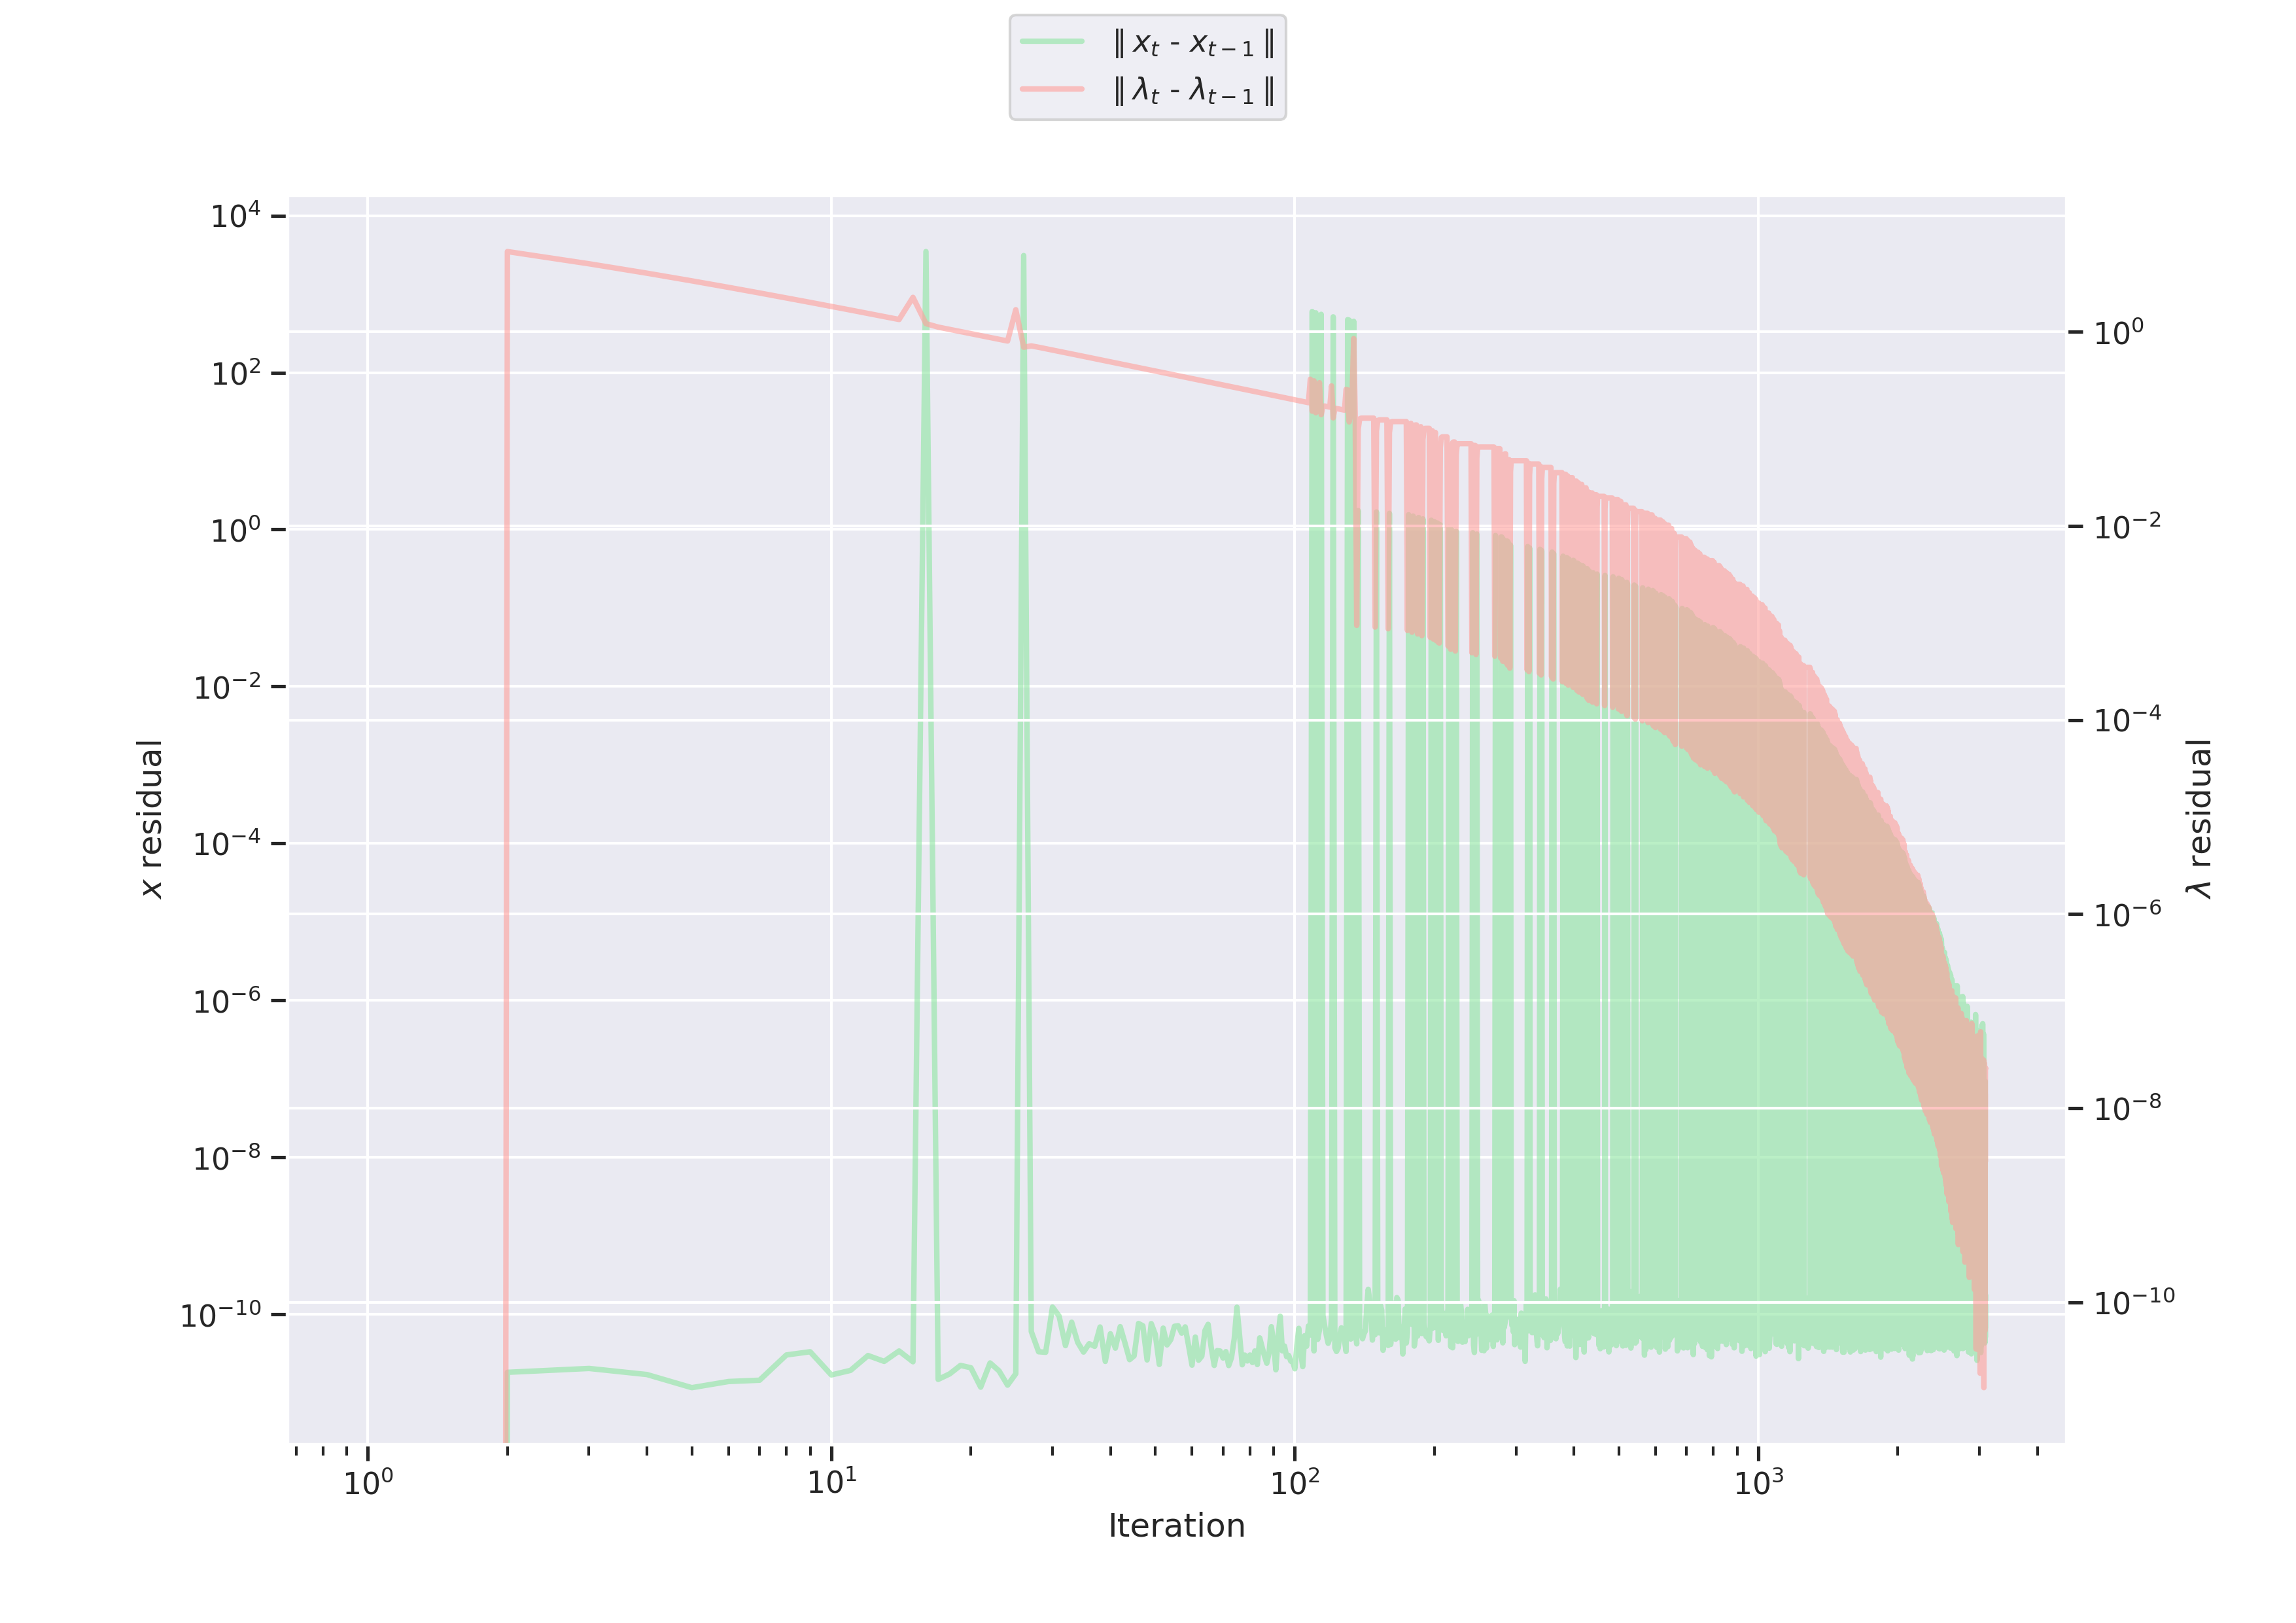
\includegraphics[scale=0.33]{pics/n=5000_K=10_lambda_rule=1.png}
%     \caption{Norms with update rule $1$, with $n=5000$ and $K=10$}
%     \label{fig:rule-1-n-5000-k-10-norm}
%   \end{minipage}  
% \end{figure}

% \begin{figure}[H]
%   \begin{minipage}{0.49\textwidth}
%     \centering
%     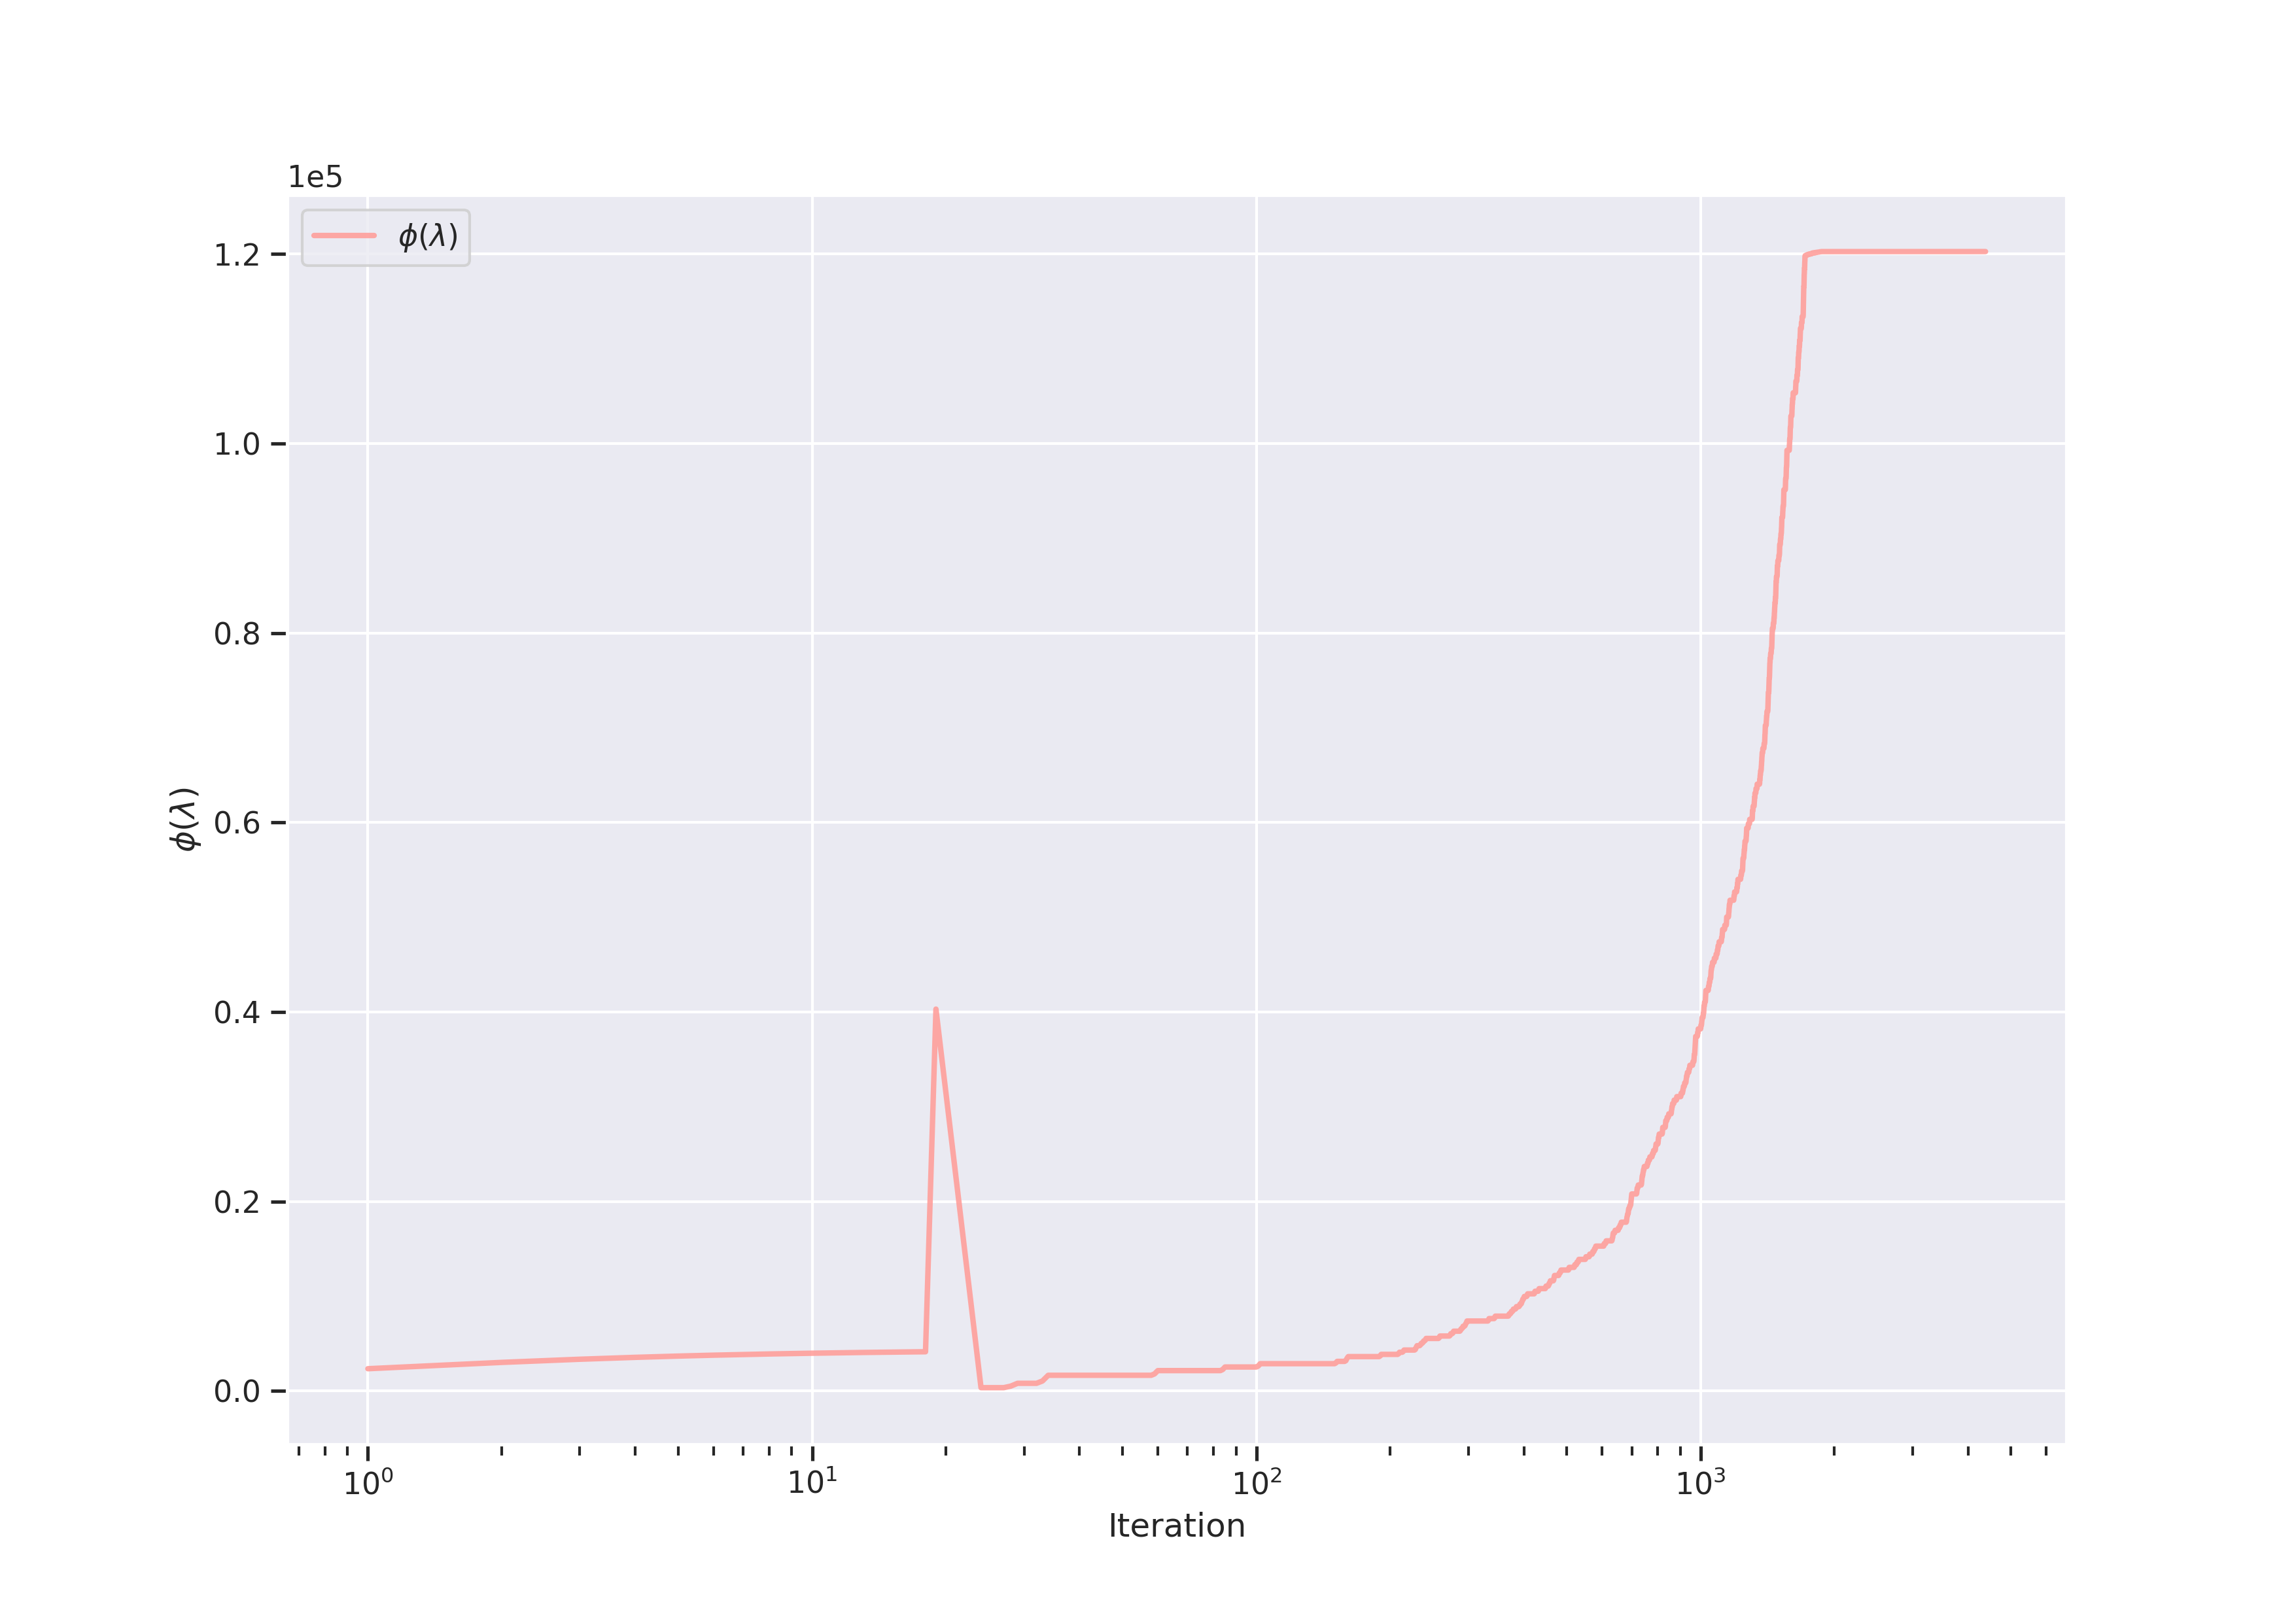
\includegraphics[scale=0.33]{pics/n=5000_K=10_dual_rule=3.png}
%     \caption{Dual value with update rule $3$, $n=5000$ and $K=10$}
%     \label{fig:rule-3-n-5000-k-10-dual}
%   \end{minipage}
%   \begin{minipage}{0.49\textwidth}
%     \centering
%     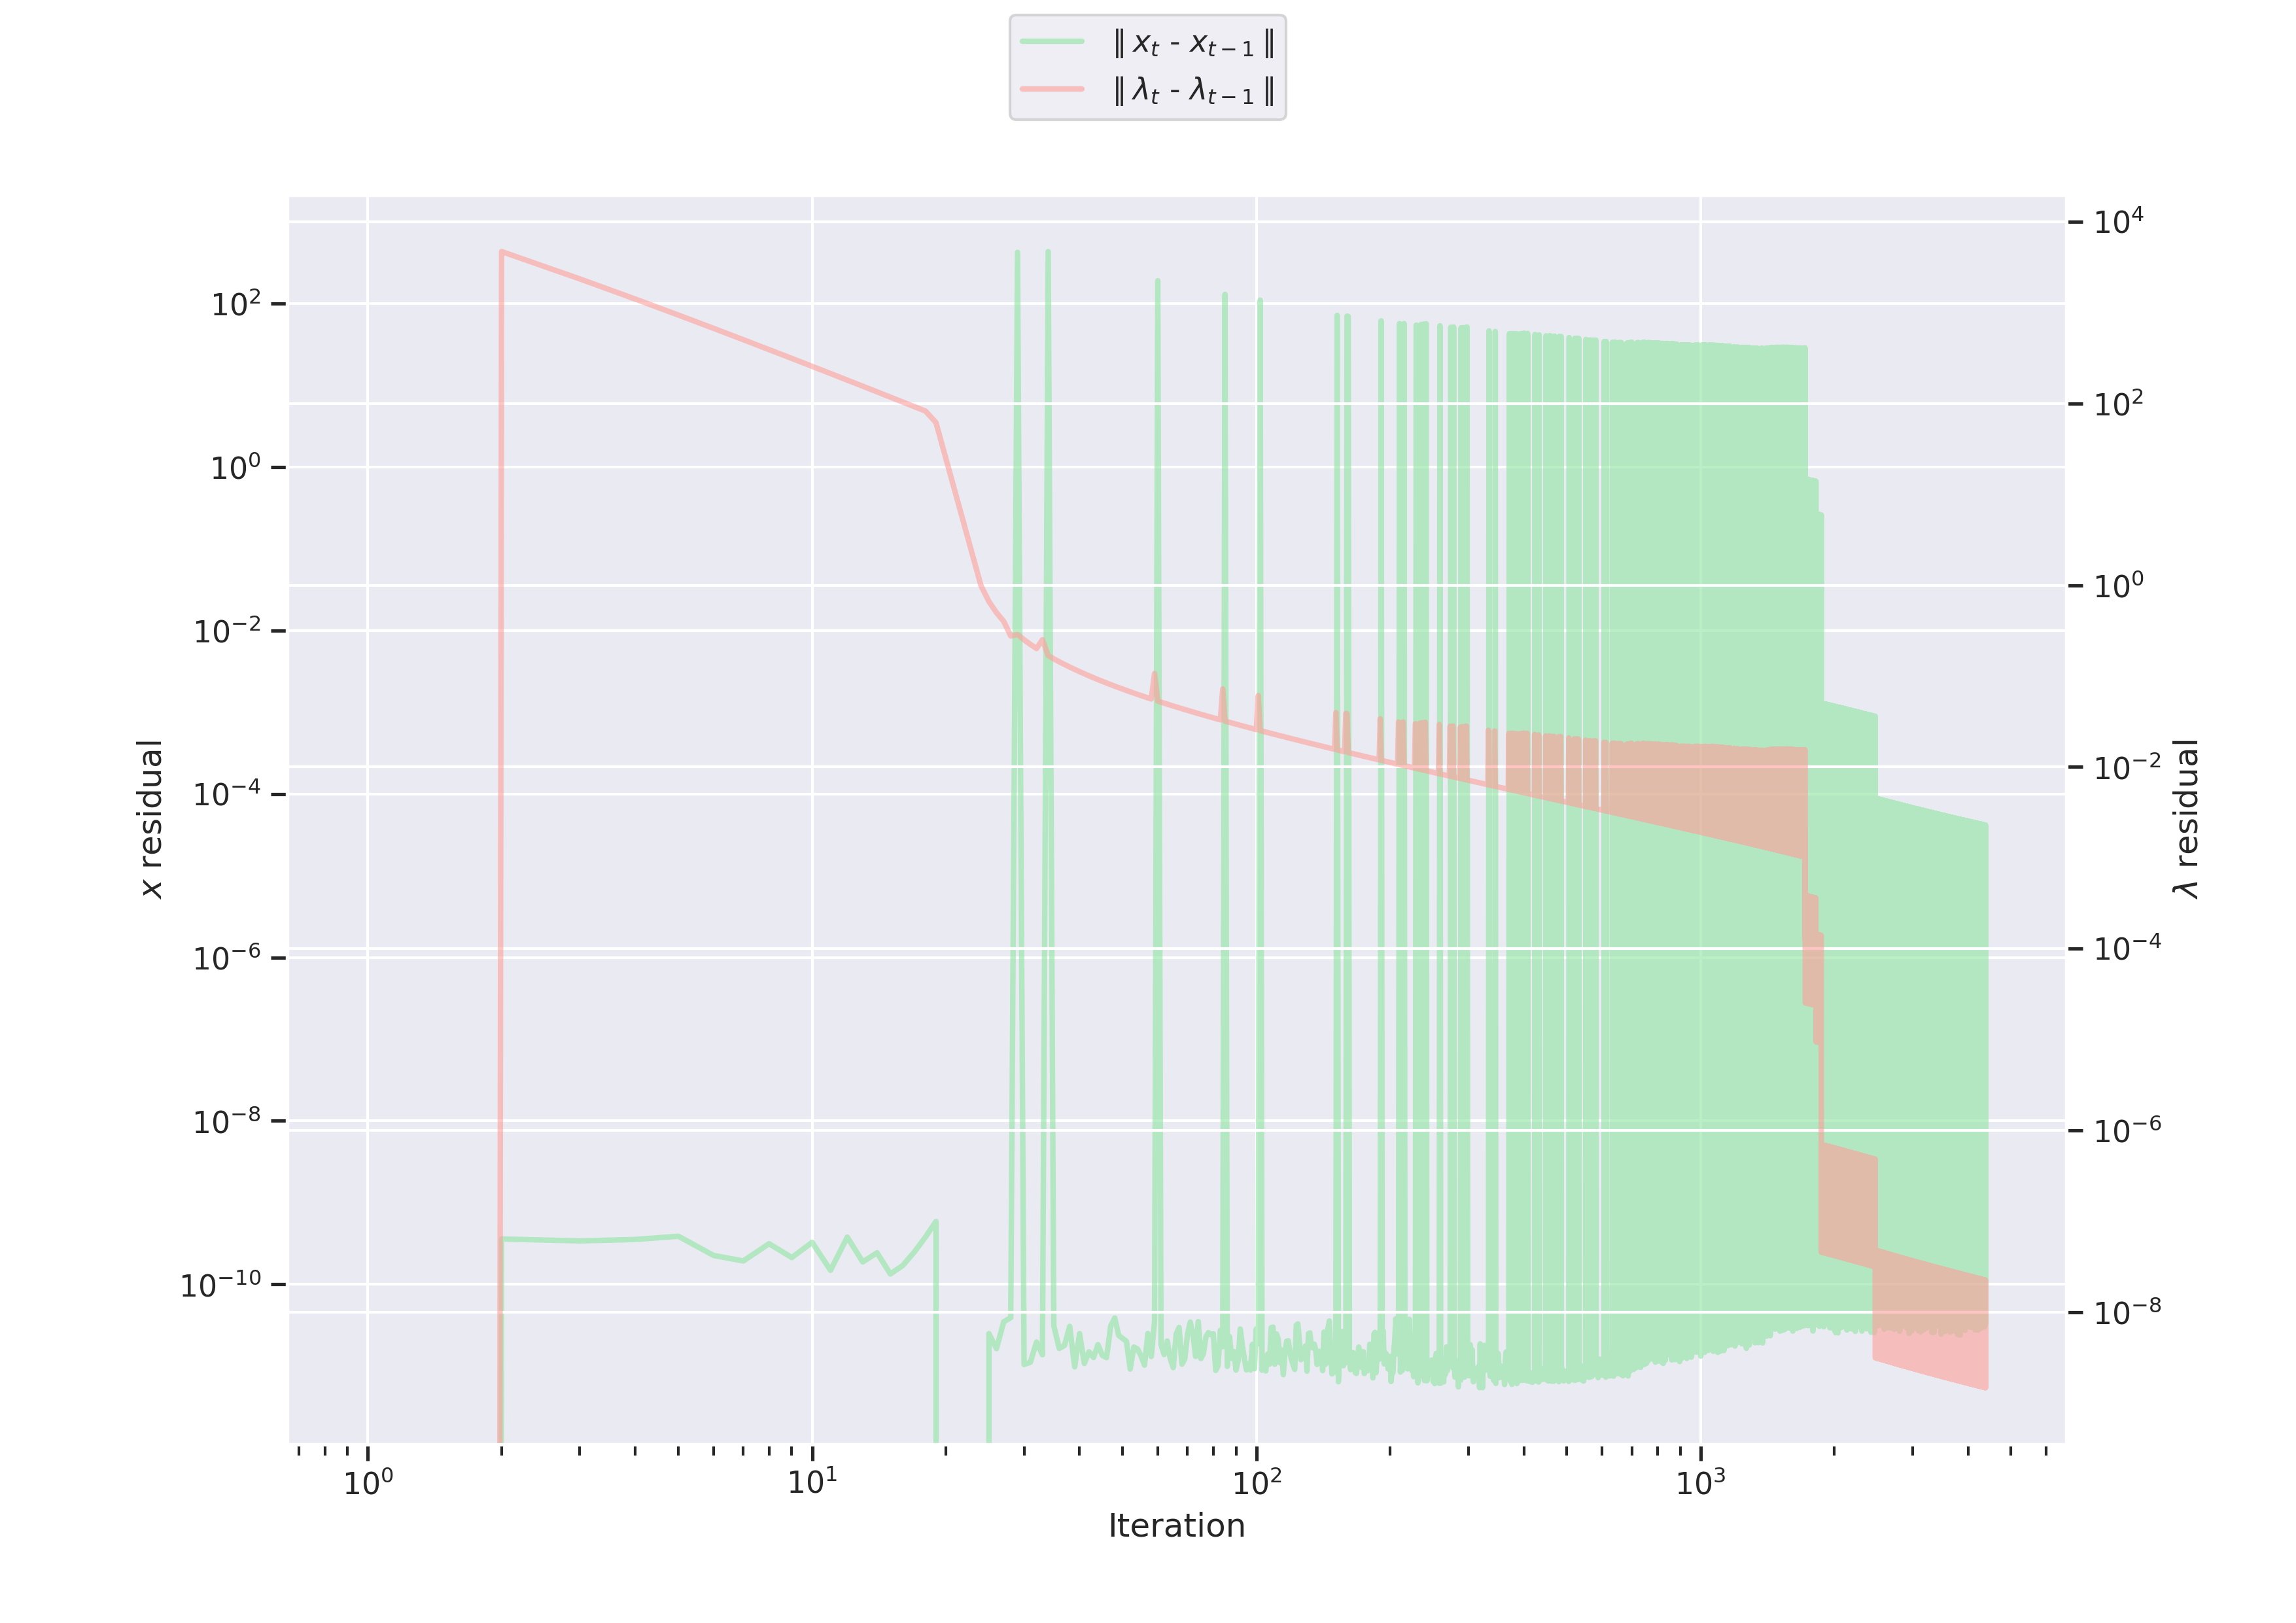
\includegraphics[scale=0.33]{pics/n=5000_K=10_lambda_rule=3.png}
%     \caption{Norms with update rule $3$, with $n=5000$ and $K=10$}
%     \label{fig:rule-3-n-5000-k-10-norm}
%   \end{minipage}  
% \end{figure}


\newpage


% \begin{table}[H]
%   \centering
%   \resizebox{\columnwidth}{!}{%
%   \begin{tabular}{| c | c | c | c | c | c | c | c | c |}
%     \hline
%     $\mathbf{Q}$ & {\itshape Update rule} & {\itshape defl} & {\itshape total iter} & {\itshape total time (sec)} & {\itshape Optimal} & {\itshape Best } $\phi(\lambda) - f(x^*)$ & {\itshape Best iteration} & {\itshape Best } $\psi(\lambda)$  \\
%     \hline
%     \multirow{6}{*}{P.D.} & \multirow{2}{*}{$1$} & {\itshape false} & $7$ & $0.0016$ & $\lambda$ & $\highlight{27.54401}$ & $2$ & $78.56617$ \\
%     \cline{3-9}
%      & & {\itshape true} & $1807$ & $0.7827$ & $\lambda$ & $39.80405$ & $32$ & $66.30613$ \\
%     \cline{2-9}
%      & \multirow{2}{*}{$2$} & {\itshape false} & $18057$ & $54.86$ & $\lambda$ & $37.33086$ & $18057$ & $68.77932$ \\ 
%     \cline{3-9}
%      & & {\itshape true} & $2915$ & $1.8307$ & $\lambda$ & $35.85367$ & $5$ & $70.25651$ \\ 
%     \cline{2-9}   
%      & \multirow{2}{*}{$3$} & {\itshape false} & $5560$ & $6.3576$ & $\lambda$ & $96.32328$ & $1$ & $9.78689$ \\
%     \cline{3-9}
%      & & {\itshape true} & $1983$ & $0.827$ & $\lambda$ & $95.91524$ & $1$ & $10.19493$ \\
%     \hline

%     \multirow{6}{*}{P.SD.} & \multirow{2}{*}{$1$} & {\itshape false} & $7024$ & $10.1979$ & $\lambda$ & $\highlight{151.9145}$ & $2$ & $0.77504$ \\
%     \cline{3-9}
%      & & {\itshape true} & $1624$ & $1.0509$ & $\lambda$ & $155.3109$ & $2$ & $-2.62131$ \\
%     \cline{2-9}
%     & \multirow{2}{*}{$2$} & {\itshape false} & $9773$ & $17.715$ & $\lambda$ & $152.63745$ & $9773$ & $0.05209$ \\ 
%     \cline{3-9}
%      & & {\itshape true} & $2$ & $0.0005$ & $\lambda$ & $152.4116$ & $2$ & $0.27795$ \\ 
%     \cline{2-9}   
%      & \multirow{2}{*}{$3$} & {\itshape false} & $4908$ & $4.7208$ & $\lambda$ & $192.6884$ & $1$ & $-39.99881$ \\
%     \cline{3-9}
%      & & {\itshape true} & $1912$ & $0.6989$ & $\lambda$ & $210.7933$ & $1$ & $-58.1038$ \\
%     \hline
%   \end{tabular}%
%   }
%   \caption{Execution with $n=50$ and $K=40$}
%   \label{tab:n-50-K-40}
% \end{table}

% \vspace{1em}

% \begin{table}[H]
%   \centering
%   \resizebox{\columnwidth}{!}{%
%   \begin{tabular}{| c | c | c | c | c | c | c | c | c |}
%     \hline
%     $\mathbf{K}$ & {\itshape Update rule} & {\itshape defl} & {\itshape total iter} & {\itshape total time (sec)} & {\itshape Optimal} & {\itshape Best } $\phi(\lambda) - f(x^*)$ & {\itshape Best iteration} & {\itshape Best } $\psi(\lambda)$  \\
%     \hline
%     \multirow{6}{*}{$20$} & \multirow{2}{*}{$1$} & {\itshape false} & $17407$ & $207.56$ & $\lambda$ & Not valid & $0$ & Not valid \\
%     \cline{3-9}
%      & & {\itshape true} & $3536$ & $13.319$ & $\lambda$ & $\highlight{18.93256}$ & $2$ & $277.3673$ \\
%     \cline{2-9}
%      & \multirow{2}{*}{$2$} & {\itshape false} & $24302$ & $396.62$ & $\lambda$ & Not valid & $0$ & Not valid \\ 
%     \cline{3-9}
%      & & {\itshape true} & $3131$ & $10.798$ & $\lambda$ & $109.6393$ & $2$ & $186.6606$ \\ 
%     \cline{2-9}   
%      & \multirow{2}{*}{$3$} & {\itshape false} & $31914$ & $893.67$ & $\lambda$ & $171.8724$ & $3$ & $124.4275$ \\
%     \cline{3-9}
%      & & {\itshape true} & $3$ & $0.021$ & $\lambda$ & $144.573$ & $3$ & $151.727$ \\
%     \hline

%     \multirow{6}{*}{$33$} & \multirow{2}{*}{$1$} & {\itshape false} & $18860$ & $265.94$ & $\lambda$ & $\highlight{578.480}$ & $2$ & $39.12439$ \\
%     \cline{3-9}
%      & & {\itshape true} & $3060$ & $11.336$ & $\lambda$ & $622.0355$ & $11$ & $-4.4311$ \\
%     \cline{2-9}
%     & \multirow{2}{*}{$2$} & {\itshape false} & $26241$ & $373.783$ & $\lambda$ & $596.7733$ & $4$ & $20.8311$ \\ 
%     \cline{3-9}
%      & & {\itshape true} & $3163$ & $11.733$ & $\lambda$ & Not valid & $0$ & Not valid \\ 
%     \cline{2-9}   
%      & \multirow{2}{*}{$3$} & {\itshape false} & $19547$ & $204.111$ & $\lambda$ & $684.7382$ & $1$ & $-67.1338$ \\
%     \cline{3-9}
%      & & {\itshape true} & $3$ & $0.028$ & $\lambda$ & $674.0635$ & $2$ & $-56.4591$ \\
%     \hline

%     \multirow{6}{*}{$50$} & \multirow{2}{*}{$1$} & {\itshape false} & $14139$ & $107.0964$ & $\lambda$ & $\highlight{4440.370}$ & $2$ & $20.7995$ \\
%     \cline{3-9}
%      & & {\itshape true} & $3499$ & $13.169$ & $\lambda$ & $4458.561$ & $1$ & $2.60828$ \\
%     \cline{2-9}
%     & \multirow{2}{*}{$2$} & {\itshape false} & $17739$ & $238.099$ & $\lambda$ & Not valid & $0$ & Not valid \\ 
%     \cline{3-9}
%      & & {\itshape true} & $2$ & $0.01$ & $\lambda$ & $4458.552$ & $1$ & $2.61751$ \\ 
%     \cline{2-9}   
%      & \multirow{2}{*}{$3$} & {\itshape false} & $11662$ & $78.604$ & $\lambda$ & $4558.096$ & $1$ & $-96.9265$ \\
%     \cline{3-9}
%      & & {\itshape true} & $3$ & $0.003$ & $\lambda$ & $4513.209$ & $2$ & $-52.0396$ \\
%     \hline

%     \multirow{6}{*}{$66$} & \multirow{2}{*}{$1$} & {\itshape false} & $15227$ & $125.117$ & $\lambda$ & $32272.27$ & $4$ & $20.2569$ \\
%     \cline{3-9}
%      & & {\itshape true} & $3093$ & $11.914$ & $\lambda$ & $32291.0$ & $3$ & $1.53456$ \\
%     \cline{2-9}
%     & \multirow{2}{*}{$2$} & {\itshape false} & $27690$ & $396.278$ & $\lambda$ & $32293.9$ & $27688$ & $-1.36491$ \\ 
%     \cline{3-9}
%      & & {\itshape true} & $11304$ & $76.041$ & $\lambda$ & $\highlight{32265.3}$ & $4$ & $27.2090$ \\ 
%     \cline{2-9}   
%      & \multirow{2}{*}{$3$} & {\itshape false} & $16347$ & $129.622$ & $\lambda$ & $32365.5$ & $1$ & $-72.9762$ \\
%     \cline{3-9}
%      & & {\itshape true} & $3307$ & $12.543$ & $\lambda$ & $32387.6$ & $1$ & $-95.0997$ \\
%     \hline

%     \multirow{6}{*}{$80$} & \multirow{2}{*}{$1$} & {\itshape false} & $4290$ & $18.700$ & $\lambda$ & $\highlight{34.4769}$ & $2$ & $56.6695$ \\
%     \cline{3-9}
%      & & {\itshape true} & $2429$ & $8.105$ & $\lambda$ & $34.7176$ & $81$ & $56.4288$ \\
%     \cline{2-9}
%     & \multirow{2}{*}{$2$} & {\itshape false} & $2$ & $0.012$ & $\lambda$ & $35.9508$ & $1$ & $55.1956$ \\ 
%     \cline{3-9}
%      & & {\itshape true} & $3163$ & $11.425$ & $\lambda$ & $35.9708$ & $3163$ & $55.1756$ \\ 
%     \cline{2-9}   
%      & \multirow{2}{*}{$3$} & {\itshape false} & $4984$ & $19.567$ & $\lambda$ & $195.0429$ & $1$ & $-103.896$ \\
%     \cline{3-9}
%      & & {\itshape true} & $3$ & $0.007$ & $\lambda$ & $194.9917$ & $1$ & $-103.845$ \\
%     \hline
%   \end{tabular}%
%   }
%   \caption{Execution with $n=100$ and positive definite $Q$}
%   \label{tab:n-100}
% \end{table}

% \begin{table}[H]
%   \centering
%   \resizebox{\columnwidth}{!}{%
%   \begin{tabular}{| c | c | c | c | c | c | c | c |}
%     \hline
%     {\itshape Update rule} & {\itshape defl} & {\itshape total iter} & {\itshape total time (sec)} & {\itshape Optimal} & {\itshape Best } $\phi(\lambda) - f(x^*)$ & {\itshape Best iteration} & {\itshape Best } $\psi(\lambda)$  \\
%     \hline
%     \multirow{2}{*}{$1$} & {\itshape false} & $14077$ & $22.044$ & $\lambda$ & Not valid & $0$ & Not valid \\
%     \cline{2-8}
%      & {\itshape true} & $2136$ & $0.596$ & $\lambda$ & $49.0422$ & $10$ & $20.4259$ \\
%     \hline
%     \multirow{2}{*}{$2$} & {\itshape false} & $14710$ & $21.287$ & $\lambda$ & $\highlight{45.1122}$ & $3$ & $24.3559$ \\ 
%     \cline{2-8}
%      & {\itshape true} & $5981$ & $4.258$ & $\lambda$ & $53.5208$ & $67$ & $15.9472$ \\ 
%     \hline   
%     \multirow{2}{*}{$3$} & {\itshape false} & $24833$ & $55.003$ & $\lambda$ & $82.5786$ & $1$ & $-13.1105$ \\
%     \cline{2-8}
%      & {\itshape true} & $2177$ & $0.470$ & $\lambda$ & $75.4582$ & $1$ & $-5.99017$ \\
%     \hline
%   \end{tabular}%
%   }
%   \caption{Execution with $n=25$, $K=13$ and positive semidefinite $Q$}
%   \label{tab:n-25}
% \end{table}


\restoregeometry

% ADD COMMENT ON RESULTS

\section{Code description}

The code is provided in Julia through package. To try it, simply open the Julia REPL inside the current folder, and launch \texttt{julia} specifying the option\\[0.2ex]
\hspace*{0.5ex}\hspace{0.5ex}\hspace{0.5ex}\texttt{--project=.}\\[0.2ex]
then enter in the \texttt{pkg} mode using \texttt{]} and launch\\[0.2ex]
\hspace*{0.5ex}\hspace{0.5ex}\hspace{0.5ex}\texttt{instantiate}\\[0.2ex]
to download the required modules. Then go back to the command line tool (simply backspace) and run\\[0.2ex]
\hspace*{0.5ex}\hspace{0.5ex}\hspace{0.5ex}\texttt{include(src/main.jl)}\\[0.2ex]
At this point you will be asked for a value of $n$ and $K$.\\
All the code is contained inside the \texttt{src} folder:
\begin{itemize}
  \item \textit{Utils.jl}: module containing some useful functions:
  \begin{itemize}
    \item \texttt{construct\_full\_matrix($Q$, $A$, $K$)}: return the entire KKT matrix;
    \item \texttt{construct\_A($K$, $n$, $I_K$)}: return the constraint matrix $A$ as described in the report;
    % \item \texttt{compute\_dualvalue($Q$,$q$,$x$,$\lambda$)}: compute the dual function $x^T Q x + q^T x - \lambda^T x$, using the solution $x$ of the lagrangian relaxation and the new $\lambda$ iterate
  \end{itemize}
  % \item \textit{ConvexSolution.jl}: module computing the off-the-shelf primal solution, containing a struct describing the problem parameters and a function to compute and return the optimal value found
  \item \textit{ADAGRAD\_Solver.jl}: module containing:
  \begin{itemize}
    \item a struct \texttt{Solver}, containing all the parameters and return value needed for the problem;
    \item functions to compute the $\lambda$/x-norm, the subgradient, the $\gamma$ value and the update rules;
    \item \texttt{my\_ADAGRAD}, which implement the algorithm derived in the report;
  \end{itemize}
  \item \textit{main.jl}: used to test all the code;
  \item \textit{solve\_prob.m}: \texttt{MATLAB} script to compute optimal primal solution using \texttt{YALMIP};
\end{itemize}
In addition, the entire project folder contains:
\begin{itemize}
  \item \textit{papers}: folder containing all the literature referenced in the bibliography;
  \item \textit{results}: folder containing all the plots and logs obtained with the experimentations values of table \ref{tab:experiments};
  \item \textit{util.sh}: a clean-up routine for the \textit{logs} and \textit{plots} produced;
  \item \textit{analyzer.py}: used to inspect the collected \textit{.csv} files and get some stats;
  \item \textit{plotter.py}: used to generate plots from the \textit{.csv} files;
\end{itemize}


\newpage

%Sets the bibliography style to UNSRT and imports the 
%bibliography file "samples.bib".
\bibliographystyle{unsrt}
\bibliography{bibliography}

\newpage

\appendix

\section{Appendix A: Updates derivations}
\label{sec:appendix}
Given a matrix $A$ of size $n \times n$, the proximal term expression of a vector $x$ of size $n\times 1$ at step $t$ is
\[
  \Psi_t(x) = \frac{1}{2} \left\langle x, A x \right\rangle  
\]

\subsection{Differentiating proximal term}
Derivation of proximal term arises from the need of obtaining the $\argmax$ $x$ of a given update function. Starting by the definition
\[
  \frac{\partial \Psi_t(x)}{\partial x} = \frac{1}{2} \frac{\partial}{\partial x} \left\langle x, A x \right\rangle  
\]
which can be rewritten in a more classical form, and the derivative is immediate
\[
  \frac{1}{2} \frac{\partial}{\partial x} x^T A x = A x
\]
% \begin{align*}
%   y = 
%   \begin{bmatrix}
%     a_{11}x_1 + a_{12}x_2 + \cdots + a_{1n}x_n \\[2ex]
%     a_{21}x_1 + a_{22}x_2 + \cdots + a_{2n}x_n \\[2ex]
%     \cdots \\
%     a_{n1}x_1 + a_{n2}x_2 + \cdots + a_{nn}x_n 
%   \end{bmatrix}
% \end{align*}
% and then expanding the scalar product we obtain
% \begin{align*}
%   \left\langle x,y \right\rangle = x_1 y_1 + x_2 y_2 + \cdots + x_n y_n
% \end{align*}
% Now we can differentiate everything w.r.t. to $x$, obtaining the closed form
% \begin{align*}
%   \frac{\partial \left\langle x,y \right\rangle}{\partial x} = 
%   \begin{bmatrix}
%     \dfrac{\partial \left\langle x,y \right\rangle}{\partial x_1} \\[3ex]
%     \dfrac{\partial \left\langle x,y \right\rangle}{\partial x_2} \\[3ex]
%     \cdots \\[3ex]
%     \dfrac{\partial \left\langle x,y \right\rangle}{\partial x_n} 
%   \end{bmatrix}
%   = 
%   \begin{bmatrix}
%     2 a_{11}x_1 + \displaystyle \sum_{\mathclap{j=1, j \neq 1}}^n a_{1j} x_j + \sum_{\mathclap{i=1, i \neq 1}}^n a_{i1} x_i \\[4ex]
%     2 a_{22}x_2 + \displaystyle \sum_{\mathclap{j=1, j \neq 2}}^n a_{2j} x_j + \sum_{\mathclap{i=1, i \neq 2}}^n a_{i2} x_i \\[4ex]
%     \cdots \\[4ex]
%     2 a_{nn}x_n + \displaystyle \sum_{\mathclap{j=1, j \neq n}}^n a_{nj} x_j + \sum_{\mathclap{i=1, i \neq n}}^n a_{in} x_i \\
%   \end{bmatrix}
% \end{align*}

\subsection{Derivation of primal-dual update}
We can now look into the detailed derivation of the update \eqref{eqn:primal-dual-update}. Starting from the equation
\[
  \lambda_{t+1} = \argmax_{\lambda \in \mathcal{X}} \{ \eta \left\langle \overline{g}_t,\lambda \right\rangle + \frac{1}{t} \Psi_t(\lambda) \} 
\]
we want to achieve the $\argmax$ over the set $\mathcal{X}$. Focusing on the maximum problem, we want to get the maximum $\lambda$, hence:
\begin{align*}
  \frac{\partial}{\partial \lambda} \eta \left\langle \overline{g}_t,\lambda \right\rangle + \frac{\partial}{\partial \lambda} \frac{1}{t} \Psi_t(\lambda) = 0 \\
  \eta\ \overline{g}_t + \frac{1}{2t} \frac{\partial}{\partial \lambda} \left\langle \lambda,H_t \lambda \right\rangle = 0 
\end{align*}  
Knowing that $H_t$ is a diagonal matrix and using the previous derivation:
\begin{align*}
  \frac{\partial}{\partial \lambda} \left\langle \lambda, H_t \lambda \right\rangle = 2\, H_t\, \lambda
\end{align*}
Substituting this into the above derivation, we get the maximum $\lambda$:
\begin{align*}
  \eta\ \overline{g}_t + \frac{1}{t} H_t\, \lambda = 0 \\
  \lambda = - H_t^{-1}\, t\, \eta\, \overline{g}_t
\end{align*}

\subsection{Derivation of composite-mirror update}
We follow the same approach also for the update \eqref{eqn:composite-mirror-update}. Starting from the definition
\[
  \lambda_{t+1} = \argmax_{\lambda \in \mathcal{X}} \{ \eta \left\langle g_t,\lambda \right\rangle + B_{\Psi_t} (\lambda,\lambda_t) \}
\]
where we remark the definition of Bregman divergence
\[
  B_{\Psi_t} (\lambda,\lambda_t) = \Psi_t(\lambda) - \Psi_t(\lambda_t) - \left\langle \nabla \Psi_t(\lambda_t),\lambda-\lambda_t \right\rangle  
\]
Also in this case, to find the $\argmax$ we derive the update formula and set it to be zero
\begin{align*}
  \frac{\partial}{\partial \lambda} \eta \left\langle g_t,\lambda \right\rangle + \frac{\partial}{\partial \lambda} B_{\Psi_t} (\lambda,\lambda_t) = 0 \\ 
  \eta\, g_t + \frac{\partial}{\partial \lambda} \left[ \Psi_t(\lambda) - \Psi_t(\lambda_t) - \left\langle \nabla \Psi_t(\lambda_t),\lambda-\lambda_t \right\rangle \right] = 0 \\
  \eta\, g_t + H_t\, \lambda - \frac{\partial}{\partial \lambda} \left\langle \nabla \Psi_t(\lambda_t),\lambda-\lambda_t \right\rangle = 0
\end{align*}
Considering the first term of the scalar product, we have to evaluate the first order taylor model of the proximal function $\Psi_t$ at the
known quantity $\lambda_t$. It is easy to see that by using the derivation in the first paragraph and the fact that $H_t$ is diagonal
\begin{align*}
  \nabla \Psi_t(\lambda_t) = \nabla \dfrac{1}{2} \left\langle \lambda_t, H_t \lambda_t \right\rangle = H_t \lambda_t
\end{align*}
Putting this into equation
\begin{align*}
  \frac{\partial}{\partial \lambda} \langle H_t \lambda_t, \lambda - \lambda_t \rangle = \frac{\partial}{\partial \lambda} \sum_{i=1}^n h_{ii} \lambda_{t,i} (\lambda_i - \lambda_{t,i})
\end{align*}
And so is easy to see that
\begin{align*}
  \dfrac{\partial}{\partial \lambda} \langle H_t \lambda_t, \lambda - \lambda_t \rangle = 
  \begin{bmatrix}
    \dfrac{\partial}{\partial \lambda_1} \langle H_t \lambda_t, \lambda - \lambda_t \rangle \\[3ex]
    \dfrac{\partial}{\partial \lambda_2} \langle H_t \lambda_t, \lambda - \lambda_t \rangle \\[3ex]
    \cdots \\[3ex]
    \dfrac{\partial}{\partial \lambda_n} \langle H_t \lambda_t, \lambda - \lambda_t \rangle
  \end{bmatrix} 
  =
  \begin{bmatrix}
    h_{11} \lambda_{t,1} \\[2ex]
    h_{22} \lambda_{t,2} \\[2ex]
    \cdots \\[2ex]
    h_{nn} \lambda_{t,n}
  \end{bmatrix}
  = 
  H_t \lambda_t
\end{align*} 
And finally putting this into the main problem, we get:
\begin{gather*}
  \eta\, g_t + H_t\, \lambda - H_t \lambda_t = 0 \quad \implies H_t\, \lambda = H_t \lambda_t - \eta\, g_t \\
  \lambda = H_t^{-1} \left[ H_t \lambda_t - \eta\, g_t \right] = \lambda_t + \eta\, H_t^{-1}\, g_t
\end{gather*}


\section{Appendix B: subgradient computation}
\label{sec:appendix_B}

Utterly following the definition, we state that $s$ is a subgradient of $\psi$ at $x$
\[
  \psi( \lambda ) \le \psi(x) + s^T (\lambda - x) \quad \forall \lambda \in \mathbb{R}^n  
\]
which reordering the term can be written as
\[
  s^T (\lambda - x) \ge \psi(\lambda) - \psi(x) \quad \forall \lambda \in \mathbb{R}^n  
\]
% We can use the rules defined for the subgradient to solve this complex inequality. By using the addition rule, we can split $\psi$ in two separate functions:
% \begin{align*}
%   \psi_1 (\lambda) = x^T Q x + q^T x \\
%   \psi_2 (\lambda) = -\lambda x
% \end{align*}
% where we immediately notice $\psi_1$ is independent from $\lambda$. We then compute the subgradient for $\psi_1$ and $\psi_2$, and then merge the solutions.\\
% Sinve we want to compute the subgradient at the point $x = \lambda_{t-1}$ (we will omit $\forall \lambda \in \mathbb{R}^n$ in the next steps)
% \begin{align*}
%   s^T (\lambda - \lambda_{t-1}) \ge \psi_1(\lambda) - \psi_1(\lambda_{t-1}) && \text{(subgradient for $\psi_1$)} \\
%   s^T (\lambda - \lambda_{t-1}) \ge \psi_2(\lambda) - \psi_2(\lambda_{t-1}) && \text{(subgradient for $\psi_2$)}
% \end{align*}   
% Using the function $\psi_1$ and $\psi_2$, we have to solve the following inequalities
% \begin{align*}
%   s^T (\lambda - \lambda_{t-1}) \ge x^T Q x + q^T x - x^T Q x - q^T x && \text{($\psi_1$)} \\
%   s^T (\lambda - \lambda_{t-1}) \ge - \lambda^T x + \lambda_{t-1}^T x && \text{($\psi_2$)} 
% \end{align*}
% Going on we immediately notice that 
% \begin{align*}
%   s^T (\lambda - \lambda_{t-1}) \ge 0 && \text{($\psi_1$)} \\
%   s^T (\lambda - \lambda_{t-1}) \ge (\lambda_{t-1}^T - \lambda^T) x && \text{($\psi_2$)} 
% \end{align*}
% where $x$ is a known quantity.

% Since we are computing the subgradient step by step on the function $\psi$, also the quantity $x$ is a known quantity. As a consequence, we can call 
% the quantity $x^T Q x + q^T x = v_2$, obtaining 
% \[
%   s^T (\lambda - \lambda_{t-1}) \ge v_2 - \lambda^T x - v_1
% \]
% Calling $v = v_2 - v_1$
% \begin{align*}
%   s^T (\lambda - \lambda_{t-1}) \ge v - \lambda^T x \\
%   s^T \ge \dfrac{v - \lambda^T x}{\lambda - \lambda_{t-1}}
% \end{align*} 
Either we can solve the above complex inequality with unknown variables $s$ and $\lambda$, or better we can apply the following reasoning. The subdifferential is the set containing all the numbers in the 
interval $\left[a,b\right]$ such that
\begin{align*}
  a = \lim_{\lambda \rightarrow \lambda_0^-} \dfrac{\psi(\lambda) - \psi(\lambda_{t-1})}{\lambda - \lambda_{t-1}} \\
  b = \lim_{\lambda \rightarrow \lambda_0^+} \dfrac{\psi(\lambda) - \psi(\lambda_{t-1})}{\lambda - \lambda_{t-1}}
\end{align*}
where the $^+$ and $^-$ portion must have a certain value greater than zero (order of $10^{-2}$).


% \section{Appendix C: \texorpdfstring{$\gamma$}{TEXT} computation}
% \label{sec:appendix_C}
% Deflection is a way to change the direction of the computed subgradient by using a convex combination
% \[
%   d^i = \gamma^i g^i + (1 - \gamma^i) d^{i-1}   
% \]
% where $g^i$ is the subgradient at iteration $i$ and $d^{i-1}$ is the direction computed at the previous step.\\
% To find the best $\gamma^i$ at iteration $i$, we could solve the problem 
% \[
%   \gamma^i \in \argmin{ \{ \| \gamma g^i + (1 - \gamma) d^{i-1} \|^2 : \gamma \in \left[0,1\right] \} }   
% \]
% Hence we have to solve
% \begin{align*}
%   \frac{\partial}{\partial \gamma} \| \gamma g^i + (1 - \gamma) d^{i-1} \|^2
% \end{align*}
% which can be rewritten as
% \begin{align*}
%   \frac{\partial}{\partial \gamma} \sum_{k=1}^n (\gamma_k g_k^i + (1 - \gamma_k) d_k^{i-1})^2 = 0
% \end{align*}
% which result in the following vector
% \begin{gather*}
%   \begin{bmatrix}
%     \dfrac{\partial}{\partial \gamma_1} \sum_{k=1}^n (\gamma_k g_k^i + (1 - \gamma_k) d_k^{i-1})^2 \\[3ex]
%     \dfrac{\partial}{\partial \gamma_2} \sum_{k=1}^n (\gamma_k g_k^i + (1 - \gamma_k) d_k^{i-1})^2 \\[3ex]
%     \vdots \\[3ex]
%     \dfrac{\partial}{\partial \gamma_n} \sum_{k=1}^n (\gamma_k g_k^i + (1 - \gamma_k) d_k^{i-1})^2
%   \end{bmatrix}
%   = \boldsymbol{0} \boldsymbol{\implies} 
%   \begin{bmatrix}
%     \dfrac{\partial}{\partial \gamma_1} (\gamma_1 g_1^i + (1 - \gamma_1) d_1^{i-1})^2 \\[3ex]
%     \dfrac{\partial}{\partial \gamma_2} (\gamma_2 g_2^i + (1 - \gamma_2) d_2^{i-1})^2 \\[3ex]
%     \vdots \\[3ex]
%     \dfrac{\partial}{\partial \gamma_n} (\gamma_n g_n^i + (1 - \gamma_n) d_n^{i-1})^2
%   \end{bmatrix}
%   = \boldsymbol{0} \boldsymbol{\implies} \\[2ex]
%   \begin{bmatrix}
%     2 (\gamma_1 g_1^i + (1 - \gamma_1) d_1^{i-1}) (g_1^i - d_1^{i-1}) \\[3ex]
%     2 (\gamma_2 g_2^i + (1 - \gamma_2) d_2^{i-1}) (g_2^i - d_2^{i-1}) \\[3ex]
%     \vdots \\[3ex]
%     2 (\gamma_n g_n^i + (1 - \gamma_n) d_n^{i-1}) (g_n^i - d_n^{i-1})
%   \end{bmatrix}
%   = \boldsymbol{0}
% \end{gather*}
% Isolating each $\gamma_i$, we obtain the following compact value for $\gamma$
% \[
%   \gamma = \dfrac{ (d^{i-1})^2 - g^i }{ (g^i - d^{i-1})^2 }  
% \]


\end{document}
